% This is the Amherst College LaTeX thesis template.
% See http://web.reed.edu/cis/help/latex.html for help. There are a
% great bunch of help pages there, with notes on
% getting started, bibtex, etc. Go there and read it if you're not
% already familiar with LaTeX.
%
% Any line that starts with a percent symbol is a comment.
% They won't show up in the document, and are useful for notes
% to yourself and explaining commands.
% Commenting also removes a line from the document;
% very handy for troubleshooting problems. -BTS

% As far as I know, this follows the requirements laid out in
% the 2002-2003 Senior Handbook. Ask a librarian to check the
% document before binding. -SN

%%
%% Preamble
%%
% \documentclass{<something>} must begin each LaTeX document
\documentclass[12pt,twoside]{amherstthesis}
% Packages are extensions to the basic LaTeX functions. Whatever you
% want to typeset, there is probably a package out there for it.
% Chemistry (chemtex), screenplays, you name it.
% Check out CTAN to see: http://www.ctan.org/
%%
\usepackage{graphicx,latexsym}
\usepackage{amsmath}
\usepackage{amssymb,amsthm}
\usepackage{longtable,booktabs,setspace}
\usepackage{chemarr} %% Useful for one reaction arrow, useless if you're not a chem major
\usepackage{rotating}

% Modified by CII
\usepackage[hyphens]{url}
\usepackage{hyperref}
\usepackage{lmodern}

% Added by CII (Thanks, Hadley!)
% Use ref for internal links
\renewcommand{\hyperref}[2][???]{\autoref{#1}}
\def\chapterautorefname{Chapter}
\def\sectionautorefname{Section}
\def\subsectionautorefname{Subsection}

\usepackage{caption}
\captionsetup{width=5in}

% \usepackage{times} % other fonts are available like times, bookman, charter, palatino

\title{Independent Component Analysis (ICA) for Blind Source Separation}
\author{Sara J. Culhane}
% The month and year that you submit your FINAL draft TO THE LIBRARY (May or December)
\date{September 17, 2017}
\division{Statistics}
\advisor{Amy Wagaman}
%If you have two advisors for some reason, you can use the following
%\altadvisor{Your Other Advisor}
%%% Remember to use the correct department!
\department{Mathematics and Statistics}
% if you're writing a thesis in an interdisciplinary major,
% uncomment the line below and change the text as appropriate.
% check the Senior Handbook if unsure.
%\thedivisionof{The Established Interdisciplinary Committee for}
% if you want the approval page to say "Approved for the Committee",
% uncomment the next line
%\approvedforthe{Committee}

% Below added by CII

%%% Copied from knitr
%% maxwidth is the original width if it's less than linewidth
%% otherwise use linewidth (to make sure the graphics do not exceed the margin)
\makeatletter
\def\maxwidth{ %
  \ifdim\Gin@nat@width>\linewidth
    \linewidth
  \else
    \Gin@nat@width
  \fi
}
\makeatother

\renewcommand{\contentsname}{Table of Contents}

\setlength{\parskip}{0pt}

\providecommand{\tightlist}{%
  \setlength{\itemsep}{0pt}\setlength{\parskip}{0pt}}

\Acknowledgements{
I would like to thank my advisor Professor Amy Wagaman for her
assistance with concepts and ideas throughout my Comprehensive Project
process as well as her dedication to excellent teaching of Statistics. I
would also like to thank Professor Horton for his commitment to the
growth Amherst Statistics program and his passion for data science. Many
thanks extended to Professor Susan Wang, Professor Jordan Crouser at
Smith and Professor Albert Kim for their invaluable courses on
Statistics and Machine Learning that impacted by studies greatly.
}

\Dedication{

}

\Preface{

}

\Abstract{
Most of statistics as well as aspects of machine learning rely on linear
models or Gaussian distributions in order to successfully model and
separate signal from noise. While our focus throughout our coursework at
Amherst has mostly been involved analysis based on known or applied
variables and distributions, Independent Component Analysis (ICA) and
other methods of Blind Source Separation (BSS) call for the
decomposition of their components with much more limited knowledge of
their distribution than we have seen previously. By identifying
independent, non-Gaussian components of a mixture with ICA, the
desired/original source can be uncovered and hidden information about
the data can be revealed. R packages like fastICA,JADE and ICA Infomax
make its application to numerous fields more efficient and usable.
}


%%
%% End Preamble
%%
%

\begin{document}

      \maketitle
  
  \frontmatter % this stuff will be roman-numbered
  \pagestyle{empty} % this removes page numbers from the frontmatter

      \begin{acknowledgements}
      I would like to thank my advisor Professor Amy Wagaman for her
      assistance with concepts and ideas throughout my Comprehensive Project
      process as well as her dedication to excellent teaching of Statistics. I
      would also like to thank Professor Horton for his commitment to the
      growth Amherst Statistics program and his passion for data science. Many
      thanks extended to Professor Susan Wang, Professor Jordan Crouser at
      Smith and Professor Albert Kim for their invaluable courses on
      Statistics and Machine Learning that impacted by studies greatly.
    \end{acknowledgements}
  
  
  % Add table of abbreviations?

      \hypersetup{linkcolor=black}
    \setcounter{tocdepth}{2}
    \tableofcontents
  
      \listoftables
  
      \listoffigures
  
      \begin{abstract}
      Most of statistics as well as aspects of machine learning rely on linear
      models or Gaussian distributions in order to successfully model and
      separate signal from noise. While our focus throughout our coursework at
      Amherst has mostly been involved analysis based on known or applied
      variables and distributions, Independent Component Analysis (ICA) and
      other methods of Blind Source Separation (BSS) call for the
      decomposition of their components with much more limited knowledge of
      their distribution than we have seen previously. By identifying
      independent, non-Gaussian components of a mixture with ICA, the
      desired/original source can be uncovered and hidden information about
      the data can be revealed. R packages like fastICA,JADE and ICA Infomax
      make its application to numerous fields more efficient and usable.
    \end{abstract}
  
  
  \mainmatter % here the regular arabic numbering starts
  \pagestyle{fancyplain} % turns page numbering back on

  \chapter*{Introduction}\label{introduction}
  \addcontentsline{toc}{chapter}{Introduction}
  
  \section{Overview : What is Blind Source Separation
  (BSS)?}\label{overview-what-is-blind-source-separation-bss}
  
  Blind Source Separation is a set of various methods in multivariate data
  analysis used to recompose unknown original sources from known data.
  These methods utilize information from the known observed sources with
  consideration of a set of unknown weights, which are then applied to the
  known observations to recover the original sources desired.In other
  words, there are always two unknowns and one known (each source is its
  own vector within the matrix).
  
  On a fundamental level, BSS attempts to solve a system of linear
  equations in which:
  
  \begin{figure}[h]
    
  
    $\bullet$ N unknown sources $s_j$ (eg. the original sources to recover) \newline
    
    
    $\bullet$ One unknown operator $\textbf{A}$ (an "un-mixing" or "de-mixing" matrix) \newline
    
    
    $\bullet$ P observed signals $x_i$ with some relation: \newline
    
    \centering $\textbf{$x = A(s)$}$
  
  \end{figure}
  
  \begin{figure}[h]
    
    \centering
  $x = A\cdot s$ 
  
  \end{figure}
  
  Where the solution to this system will be in the form:
  
  \begin{figure}[h]
    
    \centering
  $s = A^{-1}\cdot x$
  \end{figure}
  
  However, these \(s_i\) are not known values but instead a vector of
  distinct source signals, defined by their relationship to an also
  unknown operator matrix \(A\). The \(x_i\) are values that can be
  directly observed from the signal/data without decomposition. With this,
  the chosen BSS method takes the \(P\) known observations, performs a
  separation technique (also known as un-mixing or de-mixing) and outputs
  the unknown \(N\) sources that have been obscured by some unobserved
  process (i.e.~the data collection process, random noise or limits of a
  set of data in most cases). These \(y_k\) outputs should effectively
  estimate the original sources that make up the \(s\) vector(s).
  
  BSS possesses a large range of applications but can effectively uncover
  factors in data that are previously unknown or underlying the known data
  through this demixing of source signals.(Puigt, 2011)
  
  \section{ICA Generally}\label{ica-generally}
  
  \subsection{Definition: Independent Component Analysis
  (ICA)}\label{definition-independent-component-analysis-ica}
  
  Independent Component Analysis (ICA) provides a specific, efficient
  methodology to the general BSS framework described above and has been
  proven a useful application in various settings with complex data. This
  process can be referred to a generative model, as ICA determines how the
  observed data are constructed through the mixing process. (Aapo
  Hyvärinen \& Oja, 2001)
  
  While ICA follows the same basic matrix model as described above, it can
  also often also be written as:
  
  \[x = \sum_{i=1}^n a_is_i\]
  
  \subsection{Assumptions of ICA Model}\label{assumptions-of-ica-model}
  
  The two key characteristics and model requirements differentiate ICA
  from standard BSS and other methods are the following assumptions:
  
  \(\textbf{1. Assumption of statistical independence amongst the unknown source components}\)
  
  By definition, no component provides information on any of the other
  components. Independence allows the effect of each individual components
  to be isolated more easily.
  
  \(\textbf{2. Assumption of Non-Gaussianity}\):
  
  These independent components are also assumed to have strictly
  non-Gaussian distributions (or at most one independent component with a
  Gaussian distribution). Non-Gaussian is an assumption necessary as
  certain Gaussian signals may produce results where signals cannot be
  recovered. This trait distinguishes ICA from the similar structure
  method of Factor Analysis, which instead requires Gaussianity.
  (Hyvärinen \& Oja, 2000)
  
  \(\textit{Note}\)-
  
  The unknown mixing matrix will be denoted as a square for ease of
  calculation (not always the case) In this scenario, the number of IC
  will equal the number of observed mixtures (Aapo Hyvärinen \& Oja, 2001)
  
  \subsection{Ambigities of ICA Model}\label{ambigities-of-ica-model}
  
  Because of the two unknown factors (source signals and mixing matrix) :
  
  \(\bullet\) No reliable method of calculating variance of ICs exists.
  \newline
  
  \(\textbf{Solution}\) : Set the RV to have unit variance or
  \(E(s_i^2) = 1\) \newline
  
  \(\bullet\) No method of determining the order of ICs \newline
  
  \section{Primary Features of ICA (from
  Assumptions)}\label{primary-features-of-ica-from-assumptions}
  
  \subsection{Independence}\label{independence}
  
  Since independence is a fundamental condition of ICA for the
  construction of ICs , it is important to define it conceptually for
  clarity.
  
  Looking at two random variables (RV) denoted \(y_1\) and \(y_2\) in
  general, they will be independent if and only if their joint probability
  density function (pdf) can be rewritten as:
  
  \[p(y_1,y_2) = p_1(y_1)p_2(y_2)\]
  
  As seen in Probability, this property can also be extended to the
  expectation of these two functions and is denoted: \newline
  
  \[E({p_1(y_1)p_2(y_2)}) = E(p_1({y_1}))E(p_2({y_2}))\]
  
  \(\textbf{Note on Correlation and Independence}\) \newline
  
  By definition, two RV's are uncorrelated if and only if:
  
  \[E({y_1y_2}) - E({y_1})E({y_2}) = 0\]
  
  While uncorrelatedness does not necessarily imply independence,
  independent RV's will always be uncorrelated. Thus, for ICA modeling
  purposes, this property helps simplify the estimation to only
  uncorrelated values.
  
  \subsection{Non-Gaussianity and
  Measurement}\label{non-gaussianity-and-measurement}
  
  Though the Central Limit Theorem asserts that the sum of two or more
  independent RV's will tend towards a Gaussian distribution, the process
  of un-mixing actually produces non-Gaussian signals. ICA requires
  non-Gaussianity for the distributions of all source signals, as accurate
  estimation of the mixing matrix \(A\) is not even possible without
  meeting this condition.
  
  To show this, assume that the known mixing matrix \(A\) is orthogonal
  (eg. \(A^{T}A = AA^{T}= I\)) and that all of the \(s_i\) are Gaussian.
  
  Then, \(x_1\) and \(x_2\) have joint density:
  
  \[ p(x_1,x_2) = \frac{1}{2\pi}exp{(\frac{x_1^2+x_2^2}{2})}\] The
  symmetry of this joint density function makes it impossible to know the
  directional signals of the columns of matrix \(A\), and therefore, the
  matrix cannot be estimated, rendering ICA ineffective in the Gaussian
  case (although one Gaussian IC is technically allowed). (Hyvärinen \&
  Oja, 2000)
  
  \subsubsection{Kurtosis as a Measure of
  Non-gaussianity}\label{kurtosis-as-a-measure-of-non-gaussianity}
  
  One primary metric used to measure the the non-gaussianity of a random
  variable is Kurtosis. Explicitly, Kurtosis is defined as the 4th order
  cumulant:
  
  \[ kurt(y) = E(y^4) - 3(E(y^2))^2\] Since y= 1, it can be simplified to:
  
  \[ kurt(y) = E(y^4) - 3 \] Which is equivalent to the 4th moment of y.In
  a Gaussian Distribution, the 4th moment equals \(3(E(y^2))^2\)
  (Hyvärinen \& Oja, 2000)
  
  Thus,
  
  \[ kurt(y) = 3(E(y^2))^2 - 3(E(y^2))^2 = 0 \]
  
  All Gaussian distributions have Kurtosis equal to 0, and therefore, it
  is expected that most non-Gaussian distributions will usually have a
  nonzero Kurtosis with some rare exceptions. Beyond this, Kurtosis
  essentially measures the amount of deviation of RV from Gaussianity.
  (Puigt, 2011)
  
  Its use in ICA is popular due to the ease of estimation as well as its
  linearity property. This holds for two properties, assuming that \(x_1\)
  and \(x_2\) are independent:
  
  \[ kurt(x_1 + x_2) = kurt(x_1) + kurt(x_2)\]
  \[ kurt(\alpha x_1) = \alpha^4 kurt(x_1)\]
  
  \(\textbf{Issues with Kurtosis}\) - It is highly sensitive to outliers,
  as just a few extreme values can dramatically impact its calculation.
  Therefore, its application to skewed data or data with outliers that
  strongly influence the distribution may not be accurate. Given this and
  the preference for another method in R packages to be utilized later,
  kurtosis will not be discussed much further in this paper, and more
  robust methods of measuring non-Gaussianity will be explored
  instead.(Hyvärinen \& Oja, 2000)
  
  \subsubsection{Negentropy}\label{negentropy}
  
  Since Kurtosis cannot always successfully determine Non-gaussianity, the
  use of negentropy as a alternative method of estimation is typically
  preferred. Negentropy derives from the theoretical ``differential''
  entropy or level of randomness of a given variable. In general, Gaussian
  variables tend to possess the largest entropy given control for an equal
  variance condition. (Hyvärinen \& Oja, 2000)
  
  Theoretical entropy is defined for discrete and continuous respectively
  as:
  
  \[H(Y) = -\sum_{i=1}P(Y = a_i)log P(Y = a_i)\]
  
  \[H(\textbf{y}) = -\int f(\textbf{y})logf(\textbf{y})dy\] To obtain the
  desired negative differential entropy, the calculation modifies to:
  
  \[ J(\textbf{y}) = H(\textbf{y}_{gauss}) -H(\textbf{y})\]
  
  Critically in the above equation, \(\textbf{y}_\textit{gauss}\) is the
  Gaussian RV of with identical covariance as \(\textbf{y}\).
  
  It is always:
  
  \(\bullet\) Non-negative and will be zero if and only if \(\textbf{y}\)
  is Gaussian.
  
  \(\bullet\) Invariant for invertible linear transformations.
  
  In most cases, negentropy tends to be the best performing estimator of
  non-gaussianity but can be difficult or expensive to compute. However,
  the ease of computation has improved over time with technology, and thus
  the fastICA package relies on the estimator in its
  calculation.(Hyvärinen \& Oja, 2000)
  
  \subsubsection{Minimization of Mutual
  Information}\label{minimization-of-mutual-information}
  
  Though negentropy will be primarily used in subsequent examples and
  applications in this paper through fastICA, other forms of ICA
  estimation are still important to note for thoroughness purposes. A
  third commonly used estimator is the minimization of mutual information
  technique.
  
  \(\textbf{Mutual Information}\) - The MI between \(\textit{m}\) scalar
  variables \(y_i,\textit{i} = 1,..m\) is indicated by:
  
  \[ I(y_1,y_2,...,y_\textit{m}) = \sum_{i=1}^m H(y_\textit{i})-H(\textbf{y})\]
  
  This can be rewritten as the following to descibe its relationship to
  negentropy:
  
  \[ I(y_1,y_2,...,y_\textit{m}) = C- \sum_{i=1} J(y_\textit{i})\]
  
  MI measures the dependence between RV's and will be non-negative and
  zero if independent. This allows MI to be used as a criteria for ICA
  transformation by minimizing mutual information of transformed
  components. Thus, ICA can also be viewed as the minimization of mutual
  information. (Hyvärinen \& Oja, 2000)
  
  \subsubsection{Maximum Likelihood Estimation
  (MLE)}\label{maximum-likelihood-estimation-mle}
  
  A third method, MLE, serves as a similar estimation approach to the
  mutual information method for the ICA model. Particularly, the
  likelihood of the noise-free model can be formulated then used to find
  an estimate with MLE.
  
  Log-likelihood for ICA:
  
  Denote:
  
  \[ \textbf{W} = (\textbf{w}_1,...\textbf{w}_n) = \textbf{A}^{-1} \]
  
  \[ L = \sum_{t=1}^T \sum_{i=1}^n log \textit{f}_j(\textbf{w}_\textit{i}^T  \textbf{x}(t))+\textit{T}log|det\textbf{W}|\]
  
  Further simplified, this becomes:
  
  \[ \frac{1}{T} log L(\textbf{W}) = E\{\sum_{i=1}^n log p_i w_i^Tx\}) + log|det \textbf{W}|\]
  
  In this, the \(\textit{f}_i\) signify the density functions of the
  \(s_i\), which would generally be unknown but are known here.
  
  \[ \textbf{x}(t), t= 1,...,N\] are the observations of x
  
  \[ log|det\textbf{W}|\] is linear transformation of an RV and its
  density (Hyvärinen \& Oja, 2000) \newline
  
  \textbf{Connect to Infomax}
  
  A similar principle that has been used to develop ICA algorithms
  previously is Infomax (eg. the maximization of output entropy).
  
  Given a neural network with :
  
  \[ \textit{y}_i = \phi_i(\textbf{w}_i^Tx)+\textbf{n}\]
  
  Apply some function \(\textit{H()}\) and maximize:
  
  \[\textit{H}(\textbf{y}) = \textit{H}(\phi_1(\textbf{w}_1^Tx),...,\phi_n(\textbf{w}_n^Tx))\]
  \newline
  
  Maximization of mutual information will be equal to maximization of
  output entropy, for which the transformation can be written as:
  
  \[\textit{H}(\phi_1(\textbf{w}_1^Tx),...,\phi_n(\textbf{w}_n^Tx)) =\textit{H}(x)+\textit{E}\{log | det \frac{\partial F}{\partial W}(x)|\}\]
  Where:
  \[\textbf{F}(x) = (\phi_1(\textbf{b}_1^Tx),...,\phi_n(\textbf{b}_n^Tx))\]
  
  And therefore:
  
  \[\textit{E}\{log | det \frac{\partial F}{\partial W}(x)|\} = \sum_{i} \textit{E}\{log \phi_i' \textbf{w}_i^Tx\} + log|det\textbf{W}|\]
  Here the output entropy equals the likelihood, and so infomax and MLE
  are effectively equal methods for.(Aapo Hyvärinen \& Oja, 2001)
  
  \subsubsection{ICA and Projection
  Pursuit}\label{ica-and-projection-pursuit}
  
  It is important to note the relationship between ICA and Projection
  Pursuit due to some significant similarities in their processes.
  Particularly, projection pursuit also looks at multidimensional data
  with the intent to find ``interesting'' projections. Many of its key
  applications are in the data exploration phase, but often projection
  pursuit directions can successfully visualize nuanced distribution of
  the data.
  
  Beyond this, projection pursuit's goal of finding interesting data
  projections ties it directly to non-Gaussian distributions and how they
  can produce powerful visualizations of clustered data. Thus, most
  projection pursuit projections will be performed by determining the most
  non-Gaussian projects, and therefore, ICA components can be considered
  projection pursuit \(\textit{indicies}\). However, projection pursuit
  does not follow a set model with rigorous definition like ICA. If the
  specified ICA model holds, then non-Gaussainity optimization will
  generate independent components. If not, the result model can be viewed
  as a set of projection pursuit directions.(Aapo Hyvärinen \& Oja, 2001)
  
  \section{Pre-proccessing in ICA}\label{pre-proccessing-in-ica}
  
  \subsection{Centering}\label{centering}
  
  Practically speaking, centering is subtracting the expectation/mean
  vector \(\textbf{m} = E({\textbf{x}})\) from each observation to make
  \(x\) zero-mean. Centering data simplifies algorithmic processes and
  calculations.
  
  \subsection{Whitening}\label{whitening}
  
  As a concept, whitening serves to take the original data and generate
  vectors with components that are both uncorrelated and equal variance
  with theoretical notation for the covariance matrix of a whitened vector
  as stated below:
  
  \[ E(\tilde{x} \tilde{x}^T)= \textbf{I} \]
  
  Whitening, also known as \(\textit{Sphering}\), removes the scale and
  correlation structure from the \(\textbf{X}\) data matrix. In general,
  the process has been criticized for manipulating the distribution of
  data too far but still remains standard practice for pre-processing data
  for ICA.(Izenman, 2003)
  
  \section{fastICA and Other Methods}\label{fastica-and-other-methods}
  
  \subsection{Quick Look at fastICA}\label{quick-look-at-fastica}
  
  The next chapter will dig deeper in demonstrating the power of the
  fastICA R package in generating ICA models, but the key features should
  be pointed out before their application to two toy examples later.
  
  \(\textbf{Key Details}\) \newline
  
  fastICA takes the data matrix \(X\) of the model and attempts to un-mix
  components. Explicitly, this matrix is a linear combination of matrices
  \(S\) (original source signals) and \(A\) (mixing matrix) by generating
  matrix \(W\) that maximized non-Gaussianity, which is
  \(\textbf{WX = S}\) This non-Gaussian approximation is based on
  negentropy calculations discussed in prior sections, and it is used over
  kurtosis because of efficiency according to the authors of the package.
  
  Specfically for the fastICA algorithm, the \(H(\textbf{y})\) function
  options are: \newline
  
  \(\bullet G(u) = \frac{1}{\alpha}log cosh(\alpha u)\) \newline
  
  \(\bullet G(u) = -exp(u^2/2)\) \newline
  
  (J L Marchini \textless{}marchini@stats.ox.ac.uk\textgreater{} \&
  \textless{}ripley@stats.ox.ac.uk\textgreater{}, 2017)
  
  \subsection{fastICA Algorithm}\label{fastica-algorithm}
  
  \subsubsection{\texorpdfstring{``Basic'' - One Component/Unit
  Alogrithm}{Basic - One Component/Unit Alogrithm}}\label{basic---one-componentunit-alogrithm}
  
  \begin{enumerate}
  \def\labelenumi{\arabic{enumi}.}
  \item
    Choose weight vector \(\textbf{w}\)
  \item
    Let \(\textbf{w}^+\)
    =E\{\(\textbf{w}\)g(\(\textbf{w}\)\^{}T\(\textbf{x}\))\}
    -E\{\(\textbf{w}\)g'(\(\textbf{w}\)\^{}T\(\textbf{x}\))\}\(\textbf{w}\)
  \item
    Let \(\textbf{w}\) =
    \(\textbf{w}^+\)/\textbar{}\textbar{}\(\textbf{w}^+\)\textbar{}\textbar{}
  \item
    Repeat until converged (eg. old and new values of vector are same
    direction) (Hyvärinen \& Oja, 2000)
  \end{enumerate}
  
  \subsubsection{Several Units}\label{several-units}
  
  When determining multiple independent components, the vector
  \(\textbf{w}\) becomes a matrix \(\textbf{W}\) composed of vectors
  \((\textbf{w}_{1}\),\ldots{},\(\textbf{w}_{n})\) Outputs must be
  decorrelated in this scenario, else they may converge to the same value.
  This is done by iteratively subtracting \(\textbf{w}_{p+1}\) within each
  additional projection, then normalizing that same vector.
  
  \begin{enumerate}
  \def\labelenumi{\arabic{enumi}.}
  \item
    Let
    \(\textbf{w}_{p+1} = \textbf{w}_{p+1} - \sum_{j=1}^p \textbf{w}^T\textbf{w}_{j}\textbf{w}_{j}\)
  \item
    Let
    \(\textbf{w}_{p+1} = \textbf{w}_{p+1}/\sqrt{\textbf{w}_{p+1}^T \textbf{w}_{p+1}}\)
  \end{enumerate}
  
  This can also be written as:
  
  \begin{enumerate}
  \def\labelenumi{\arabic{enumi}.}
  \item
    Let \(\textbf{W} = \textbf{W}/\sqrt{||\textbf{WW}^T||}\)
  \item
    Let \(\textbf{W}\) =
    \((3/2)*\)\(\textbf{W}\)-\((1/2)\)*\(\textbf{W}\textbf{W}^T\textbf{W}\)
    (Hyvärinen \& Oja, 2000)
  \end{enumerate}
  
  \subsection{Key Properties of fastICA}\label{key-properties-of-fastica}
  
  These are the key properties of fastICA that make it an efficient and
  effective ICA modeling method.
  
  \begin{enumerate}
  \def\labelenumi{\arabic{enumi}.}
  \item
    Cubic/quadratic convergence leads to faster convergences than linear
    methods
  \item
    No step size parameters
  \item
    No estimate distribution needs to be chosen
  \item
    Can choose suitable non-linearity
  \item
    Components can be done one by one, reducing computational expense
  \item
    Neural algorithm: parallel, distributed, computationally simple, and
    requires little memory
  \end{enumerate}
  
  \subsection{Arguments in the fastICA
  function}\label{arguments-in-the-fastica-function}
  
  fastICA (R implementation) also employs several different technical
  arguments in its function that must be understood in order to interrupt
  the results of its output rigorously.
  
  \(X\) simply the data matrix of interest
  
  \(n.comp\) Number of components to be extracted
  
  \(alg.typ\) : \newline
  
  \(1.\) if == ``parallel'' - components are extracted
  simultaneously(default)
  
  \(2.\) if == ``deflation'' - components are extracted one at a time
  \newline
  
  \(fun\) Function form of G to use (see above)
  
  \(alpha\) Constant range{[}1,2{]} used in approx. to neg-entropy when
  fun == ``logcosh''
  
  \(method\) : \newline
  
  \(1\) if == ``R'' then computations are done exclusively in R
  
  \(2.\) if == ``C'' then C code is used to perform computations (runs
  faster) \newline
  
  \(row.norm\) logical value indicating whether rows of X should be
  standardized
  
  \(maxit\) Maximum number of iterations
  
  \(tol\) A positive scalar giving tolerance at which the un-mix is
  considered to have converged
  
  \(verbose\) level of output
  
  \(w.init\) Initialized un-mixing matrix of dim(n.comp,n.comp) if Null
  matrix of RV's used
  
  \subsection{JADE and Infomax}\label{jade-and-infomax}
  
  Although fastICA has largely become the primary R package for ICA
  modeling, JADE and Infomax methods are also available to perform the
  same task. In subsequent sections, their effectiveness will be evaluated
  in relation to fastICA. \newline
  
  \(\textbf{JADE}\) -
  
  Uses \(\textit{Joint Approximate Diagonalization of Eigenmatrices}\)
  (JADE) derived by Cardoso and Souloumiac in 1993. This approach involves
  finding an orthogonal rotation matrix R that diagonalizes the cumulant
  array of source signals. (Helwig, 2015) \newline
  
  Particularly, the original Cardoso paper describes the algorithm in 4
  steps: \newline
  
  \(\textbf{1}\) Create sample covariance \(\hat{R}_x\) and compute
  whitening matrix \(\hat{W}\) \newline
  
  \(\textbf{2}\) Create sample of 4th-order cumulants of whitening;
  compute significant eigenpairs \newline
  
  \(\textbf{3}\) Jointly diagonialize the set with unitary matrix \newline
  
  \(\textbf{4}\) Estimate A with \(\hat{A} =\hat{W}\hat{U}\) \newline
  
  (Cardoso \& Souloumiac, 1993) \newline
  
  \(\textbf{Infomax}\) - \newline
  
  Infomax also utilizes the orthogonal rotation matrix R that maximizes
  the joint entropy of a non-linear function of the estimated source
  signals and is derived from Bell and Sejnowski's 1995 paper
  \(\textit{An Information-Maximization Approach to Blind Separation and Blind Deconvolution}\).(Helwig,
  2015)
  
  \chapter{Chapter 1: Toy Examples and
  Simulation}\label{chapter-1-toy-examples-and-simulation}
  
  \subsection{Simple Example: Two Random uniform
  Distributions}\label{simple-example-two-random-uniform-distributions}
  
  To demonstrate effectiveness of ICA at decomposing source signals and to
  develop a better understanding of the process conceptually,a simple toy
  example will be used. The``unknown'' source components in this model are
  just two random uniform variables in the matrix \(S\), distorted by some
  arbitrary ``unknown.'' \newline
  
  Here the mixing matrix is \(A\)
  
  \[A = \begin{bmatrix} 1 & 1 \\ -1 & 3  \end{bmatrix}\] .
  
  The known observations is the product of these two matrices, or matrix
  \(X\). \newline
  
  To test ICA, apply fastICA to this simple model and generate 5 plots:
  \newline
  
  \(\textbf{1.}\) The pre-processed data \newline
  
  \(\textbf{2.}\) Principle Component Analysis (PCA - for comparison to a
  different component based model) \newline
  
  \(\bullet\) \$\textbf{ICA components} \newline 
  
  \(\textbf{3.}\) fastICA
  
  \(\textbf{4.}\) JADE method
  
  \(\textbf{5.}\) Infomax
  
  With the Random Uniform case, the distribution of signals is known to be
  two random uniform vectors, so it is desired to show that the ICA method
  can unmix the mixture matrix back into the original, known S. Therefore,
  the plot ICA components should look very similar to the plot of the two
  random uniforms.
  
  (This test case has been adapted from the fastICA package Example 1)
  
  (see J L Marchini \textless{}marchini@stats.ox.ac.uk\textgreater{} \&
  \textless{}ripley@stats.ox.ac.uk\textgreater{}, 2017)
  
  \begin{Shaded}
  \begin{Highlighting}[]
  \KeywordTok{set.seed}\NormalTok{(}\DecValTok{10}\NormalTok{) }
  \CommentTok{# Original source signals (usually unknown)}
  \NormalTok{S <-}\StringTok{ }\KeywordTok{matrix}\NormalTok{(}\KeywordTok{runif}\NormalTok{(}\DecValTok{10000}\NormalTok{), }\DecValTok{1000}\NormalTok{, }\DecValTok{2}\NormalTok{) }
  \CommentTok{# Mixing matrix (usually unknown)}
  \NormalTok{A <-}\StringTok{ }\KeywordTok{matrix}\NormalTok{(}\KeywordTok{c}\NormalTok{(}\DecValTok{1}\NormalTok{, }\DecValTok{1}\NormalTok{, }\OperatorTok{-}\DecValTok{1}\NormalTok{, }\DecValTok{3}\NormalTok{), }\DecValTok{2}\NormalTok{, }\DecValTok{2}\NormalTok{, }\DataTypeTok{byrow =} \OtherTok{TRUE}\NormalTok{) }
  \CommentTok{# "Observed" mixture - always known}
  \NormalTok{X <-}\StringTok{ }\NormalTok{S }\OperatorTok\StringTok{ }\NormalTok{A }
  
  \CommentTok{#ICA}
  \NormalTok{a <-}\StringTok{ }\KeywordTok{fastICA}\NormalTok{(X, }\DecValTok{2}\NormalTok{, }\DataTypeTok{alg.typ =} \StringTok{"parallel"}\NormalTok{, }\DataTypeTok{fun =} \StringTok{"logcosh"}\NormalTok{, }\DataTypeTok{alpha =} \DecValTok{1}\NormalTok{, }
               \DataTypeTok{method =} \StringTok{"C"}\NormalTok{, }\DataTypeTok{row.norm =} \OtherTok{FALSE}\NormalTok{, }\DataTypeTok{maxit =} \DecValTok{200}\NormalTok{, }
               \DataTypeTok{tol =} \FloatTok{0.0001}\NormalTok{, }\DataTypeTok{verbose =} \OtherTok{TRUE}\NormalTok{)}
  
  \CommentTok{#JADE}
  \NormalTok{b <-}\StringTok{ }\KeywordTok{icajade}\NormalTok{(X,}\DecValTok{2}\NormalTok{,}\DataTypeTok{center=}\OtherTok{TRUE}\NormalTok{,}\DataTypeTok{maxit=}\DecValTok{200}\NormalTok{,}\DataTypeTok{tol=}\FloatTok{0.0001}\NormalTok{)}
  
  \CommentTok{#Infomax}
  \NormalTok{c <-}\StringTok{ }\KeywordTok{icaimax}\NormalTok{(X,}\DataTypeTok{nc=}\DecValTok{2}\NormalTok{,}\DataTypeTok{center=}\OtherTok{TRUE}\NormalTok{,}\DataTypeTok{maxit=}\DecValTok{200}\NormalTok{,}\DataTypeTok{tol=}\FloatTok{0.0001}\NormalTok{,}\DataTypeTok{alg=}\StringTok{"newton"}\NormalTok{,}\DataTypeTok{fun=}\StringTok{"log"}\NormalTok{)}
  \end{Highlighting}
  \end{Shaded}
  
  \begin{center}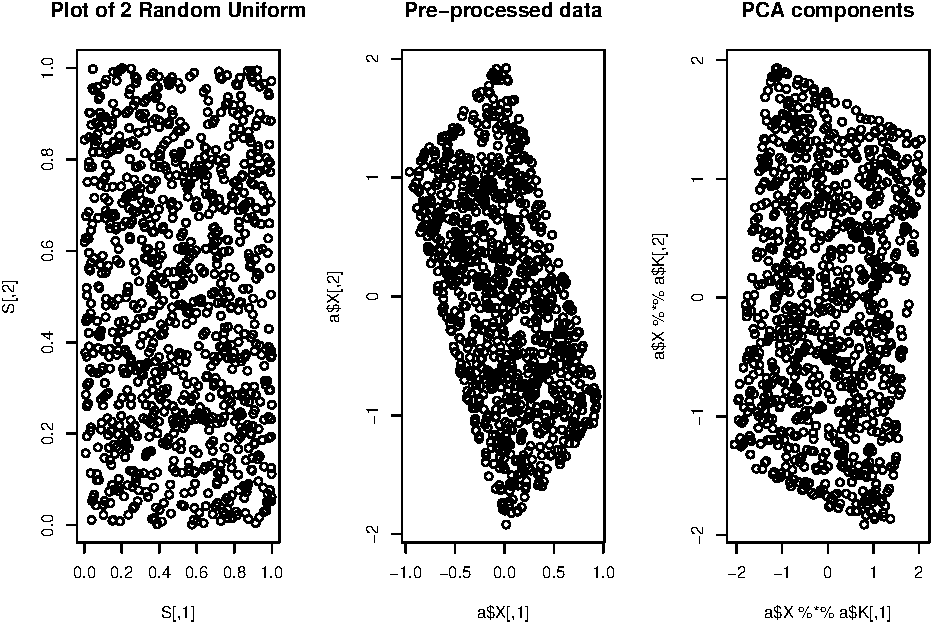
\includegraphics{ICAStatsComps_files/figure-latex/unnamed-chunk-3-1} \end{center}
  
  \begin{center}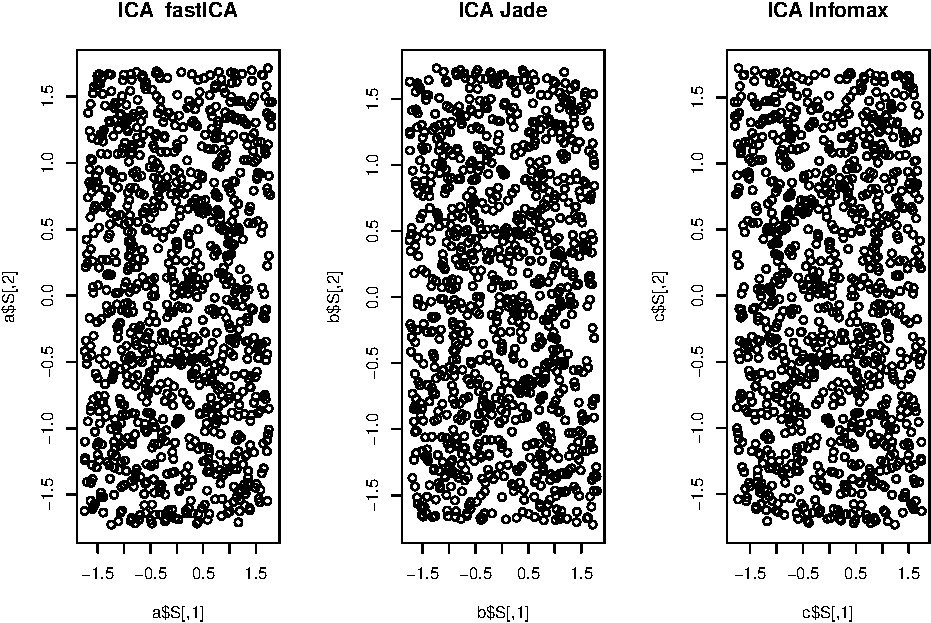
\includegraphics{ICAStatsComps_files/figure-latex/unnamed-chunk-3-2} \end{center}
  
  \subsubsection{Plot Interpretation}\label{plot-interpretation}
  
  Looking at these plots, the pre-processed data (plot of the constructed
  X) is rotated and no signals are clear from it.
  
  PCA appears to have flattened the data slightly and creates almost a
  mirror of the original data, but the true signals from the distributions
  still do not appear completely evident. PCA does not effectively
  separate sources given how it rotates data.
  
  However, looking at the ICA transformation,the shape of the original
  uniform distribution clearly forms after the decomposition. ICA was able
  to recover the original signals quite easily in this simple simulation.
  The results for all 3 ICA packages (JADE,Infomax and fastICA) appear to
  produce approximately the same plots for this example.
  
  \subsubsection{Congurence Coefficient of Source
  Signals}\label{congurence-coefficient-of-source-signals}
  
  To get an idea of the underlying differences between these methods, the
  absolute maximum column value of the congruence coefficient of each
  un-mixing matrix can be calculated.
  
  Tucker's Congruency Coefficient compares uncentered correlation between
  the columns of two matrices of the same dimensions. The absolute value
  of max column of this coefficient is then taken.
  
  \begin{Shaded}
  \begin{Highlighting}[]
  \NormalTok{colMax <-}\StringTok{ }\ControlFlowTok{function}\NormalTok{(data) }\KeywordTok{sapply}\NormalTok{(data, max, }\DataTypeTok{na.rm =} \OtherTok{TRUE}\NormalTok{)[}\DecValTok{1}\NormalTok{] }\CommentTok{#Function to find colMax }
  \NormalTok{Fast1 <-}\StringTok{ }\KeywordTok{colMax}\NormalTok{(}\KeywordTok{abs}\NormalTok{(}\KeywordTok{congru}\NormalTok{(S,a}\OperatorTok{$}\NormalTok{S)))}
  \NormalTok{JADE1 <-}\StringTok{ }\KeywordTok{colMax}\NormalTok{(}\KeywordTok{abs}\NormalTok{(}\KeywordTok{congru}\NormalTok{(S,b}\OperatorTok{$}\NormalTok{S)))}
  \NormalTok{Info1 <-}\StringTok{ }\KeywordTok{colMax}\NormalTok{(}\KeywordTok{abs}\NormalTok{(}\KeywordTok{congru}\NormalTok{(S,c}\OperatorTok{$}\NormalTok{S)))}
  \end{Highlighting}
  \end{Shaded}
  
  \begin{verbatim}
     Method Absolute Max Congruence Coef
  1 fastICA                  0.007352430
  2    JADE                  0.010033080
  3 Infomax                  0.009346984
  \end{verbatim}
  
  With just one dataset in this toy example,the results from the absolute
  maximum congruence coefficient test do not indicate accurately which
  algorithm will perform best overall. A higher value will indicate more
  similarities between the actual source matrix and the S generated by an
  ICA method. Here JADE and Infomax seem to perform better, but this value
  needs to be replicated and tested with more noise to determine if
  fastICA is truly less effective on multiple datasets. This computation
  will be done with the later simulation.
  
  \subsection{(More) Complex Example: The Cocktail Party
  Problem}\label{more-complex-example-the-cocktail-party-problem}
  
  The most common example used to explain and motivate the use of ICA (or
  any type of BSS) is the ``Cocktail Party Problem.''
  
  Two (or more) microphones are placed in a room where to different people
  are speaking at the same time. Each microphone signal is defined as
  \(x_1(t)\) and \(x_2(t)\), with some observed (i.e.~known) amplitudes
  \(x_1\) and \(x_2\) with time as an index. The unknown speech signals of
  the speakers are denoted \(s_1(t)\) and \(s_2(t)\) to make up the
  following system of equations:
  
  \[ x_1(t) = a_{11}s_1 +a_{12}s_2 \]
  
  \[ x_2(t) = a_{21}s_1 +a_{22}s_2 \]
  
  This can also be rewritten as:
  
  \[x_i = \begin{bmatrix} x_1 \\ x_2 \end{bmatrix}\]
  \[s_i = \begin{bmatrix} s_1 \\ s_2 \end{bmatrix}\]
  \[A = \begin{bmatrix} a_{11} & a_{12} \\ a_{21} & a_{22}  \end{bmatrix}\]
  
  If the weighted \(a_{ij}\) was known, this problem could be easily
  solved but because it is not, ICA becomes a necessary tool
  
  \subsubsection{Example with Cocktail Party
  Data}\label{example-with-cocktail-party-data}
  
  A test example and simulation can be generated using the CPPdata from
  the JADE package that contains 50,000 observations from 4 different
  microphones. (Klaus Nordhausen, 2017)
  
  A smaller sample of 10,000 is take here for graphical and calculation
  purposes.
  
  \begin{Shaded}
  \begin{Highlighting}[]
  \KeywordTok{set.seed}\NormalTok{(}\DecValTok{40}\NormalTok{)}
  \NormalTok{dat <-}\StringTok{ }\NormalTok{CPPdata[}\KeywordTok{sample}\NormalTok{(}\DecValTok{10000}\NormalTok{),]}
  \NormalTok{dat <-}\StringTok{ }\KeywordTok{mutate}\NormalTok{(dat, }\DataTypeTok{count=} \DecValTok{1}\OperatorTok{:}\KeywordTok{nrow}\NormalTok{(dat))}
  \KeywordTok{colnames}\NormalTok{(dat) <-}\StringTok{ }\KeywordTok{c}\NormalTok{(}\StringTok{"x"}\NormalTok{,}\StringTok{"y"}\NormalTok{,}\StringTok{"z"}\NormalTok{,}\StringTok{"t"}\NormalTok{, }\StringTok{"count"}\NormalTok{) }\CommentTok{# sample to reduce noise}
  \NormalTok{dat <-}\StringTok{ }\KeywordTok{mutate}\NormalTok{(dat, }\DataTypeTok{count=} \DecValTok{1}\OperatorTok{:}\KeywordTok{nrow}\NormalTok{(dat))}
  \end{Highlighting}
  \end{Shaded}
  
  \subsubsection{Original Source Signals}\label{original-source-signals}
  
  Unlike with the Random Uniform example, the true source signal matrix is
  unknown and the only information provided is the observed data. Because
  of this, it makes sense to look at each column (different microphone)
  separately as a starting point.
  
  \begin{center}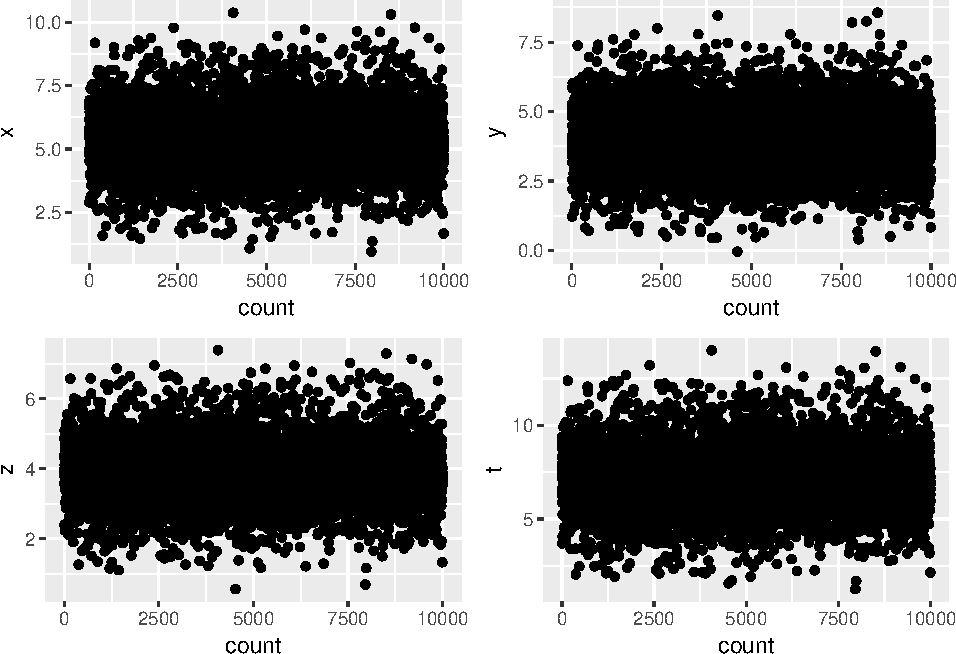
\includegraphics{ICAStatsComps_files/figure-latex/unnamed-chunk-7-1} \end{center}
  
  Each microphone has unique signal even to the point of quite variable
  means.
  
  \begin{Shaded}
  \begin{Highlighting}[]
  \NormalTok{m <-}\StringTok{ }\KeywordTok{fastICA}\NormalTok{(dat,}\DecValTok{2}\NormalTok{,}\DataTypeTok{alg.typ =} \StringTok{"parallel"}\NormalTok{, }\DataTypeTok{fun =} \StringTok{"logcosh"}\NormalTok{, }\DataTypeTok{alpha =} \DecValTok{1}\NormalTok{, }
               \DataTypeTok{method =} \StringTok{"C"}\NormalTok{, }\DataTypeTok{row.norm =} \OtherTok{FALSE}\NormalTok{, }\DataTypeTok{maxit =} \DecValTok{200}\NormalTok{, }
               \DataTypeTok{tol =} \FloatTok{0.0001}\NormalTok{, }\DataTypeTok{verbose =} \OtherTok{TRUE}\NormalTok{)}
  \end{Highlighting}
  \end{Shaded}
  
  \begin{verbatim}
  Centering
  Whitening
  Symmetric FastICA using logcosh approx. to neg-entropy function
  Iteration 1 tol=0.005382
  Iteration 2 tol=0.000005
  \end{verbatim}
  
  \begin{Shaded}
  \begin{Highlighting}[]
  \NormalTok{n <-}\StringTok{ }\KeywordTok{icajade}\NormalTok{(dat,}\DecValTok{4}\NormalTok{,}\DataTypeTok{center=}\OtherTok{TRUE}\NormalTok{,}\DataTypeTok{maxit=}\DecValTok{200}\NormalTok{,}\DataTypeTok{tol=}\FloatTok{0.0001}\NormalTok{)}
  \NormalTok{o <-}\StringTok{ }\KeywordTok{icaimax}\NormalTok{(dat,}\DataTypeTok{nc=}\DecValTok{4}\NormalTok{,}\DataTypeTok{center=}\OtherTok{TRUE}\NormalTok{,}\DataTypeTok{maxit=}\DecValTok{200}\NormalTok{,}\DataTypeTok{tol=}\FloatTok{0.0001}\NormalTok{,}\DataTypeTok{alg=}\StringTok{"newton"}\NormalTok{,}\DataTypeTok{fun=}\StringTok{"log"}\NormalTok{)}
  \end{Highlighting}
  \end{Shaded}
  
  \begin{center}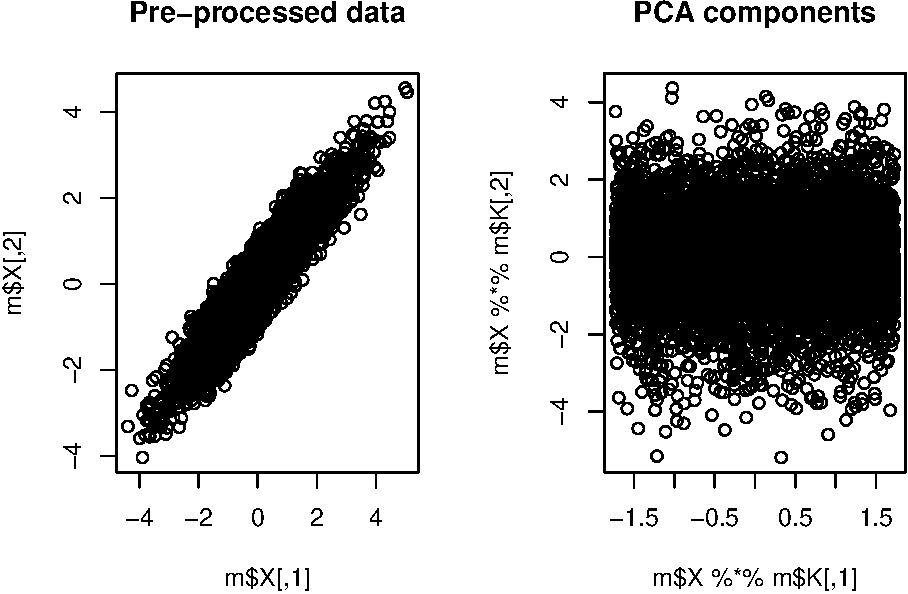
\includegraphics{ICAStatsComps_files/figure-latex/unnamed-chunk-9-1} \end{center}
  
  \begin{center}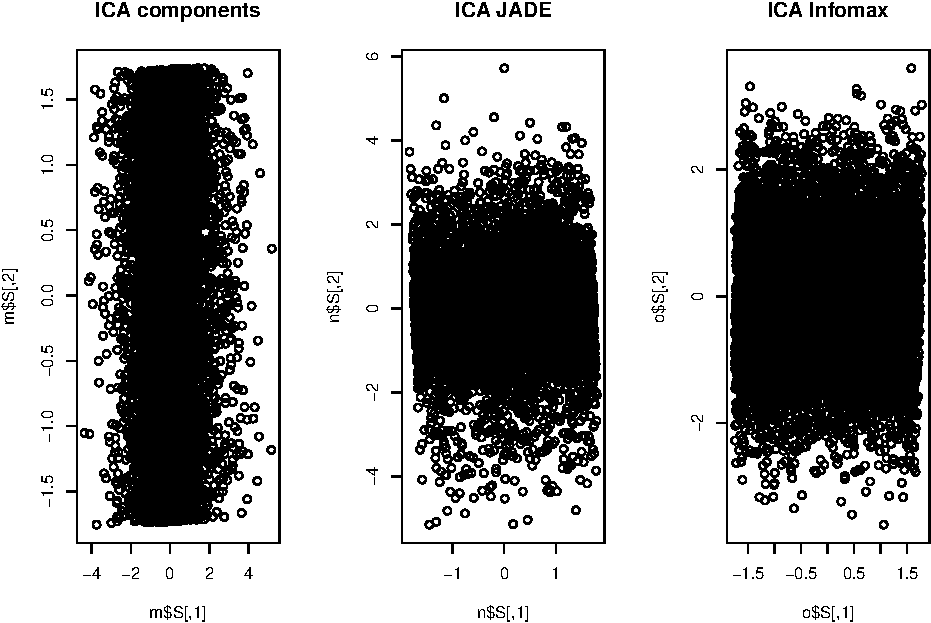
\includegraphics{ICAStatsComps_files/figure-latex/unnamed-chunk-9-2} \end{center}
  
  \subsubsection{Plot Interpretation}\label{plot-interpretation-1}
  
  Again, the data appears to have a highly rotated set of pre-processed
  data and a PCA rotation that only transforms the data enough to separate
  the mixture ever so slightly.
  
  With ICA, a full rotation and a much cleaner shape begin to form, almost
  diamond-like. Like with the random uniform example, the superior
  performance of any one of the three ICA methods is not identifiable just
  from these primitive plots of the model.
  
  Of note with the ICA algorithms example is the ``nc'' (number of
  components) input of the function for each of these different methods.
  Particularly, both the JADE and Infomax produce similar plots at
  \(nc=4\), which makes sense as the dataset \(CPPdata\) has observations
  from 4 microphones. However, to generate a similar plot for fastICA,
  \(nc=2\) was used. The results for \(nc=4\) with ICA appear as below
  (JADE and Infomax shown at \(nc=2\)) for reverse comparison.
  
  \begin{Shaded}
  \begin{Highlighting}[]
  \NormalTok{S <-}\StringTok{ }\KeywordTok{matrix}\NormalTok{(}\KeywordTok{runif}\NormalTok{(}\DecValTok{10000}\NormalTok{), }\DecValTok{1000}\NormalTok{, }\DecValTok{2}\NormalTok{)}
  \NormalTok{A <-}\StringTok{ }\KeywordTok{matrix}\NormalTok{(}\KeywordTok{c}\NormalTok{(}\DecValTok{1}\NormalTok{, }\DecValTok{1}\NormalTok{, }\OperatorTok{-}\DecValTok{1}\NormalTok{, }\DecValTok{3}\NormalTok{), }\DecValTok{2}\NormalTok{, }\DecValTok{2}\NormalTok{, }\DataTypeTok{byrow =} \OtherTok{TRUE}\NormalTok{)}
  \NormalTok{X <-}\StringTok{ }\NormalTok{S }\OperatorTok\StringTok{ }\NormalTok{A}
  \NormalTok{m <-}\StringTok{ }\KeywordTok{fastICA}\NormalTok{(dat,}\DecValTok{4}\NormalTok{,}\DataTypeTok{alg.typ =} \StringTok{"parallel"}\NormalTok{, }\DataTypeTok{fun =} \StringTok{"logcosh"}\NormalTok{, }\DataTypeTok{alpha =} \DecValTok{1}\NormalTok{, }
               \DataTypeTok{method =} \StringTok{"C"}\NormalTok{, }\DataTypeTok{row.norm =} \OtherTok{FALSE}\NormalTok{, }\DataTypeTok{maxit =} \DecValTok{200}\NormalTok{, }
               \DataTypeTok{tol =} \FloatTok{0.0001}\NormalTok{, }\DataTypeTok{verbose =} \OtherTok{TRUE}\NormalTok{)}
  \NormalTok{n <-}\StringTok{ }\KeywordTok{icajade}\NormalTok{(dat,}\DecValTok{2}\NormalTok{,}\DataTypeTok{center=}\OtherTok{TRUE}\NormalTok{,}\DataTypeTok{maxit=}\DecValTok{200}\NormalTok{,}\DataTypeTok{tol=}\FloatTok{0.0001}\NormalTok{)}
  
  \NormalTok{o <-}\StringTok{ }\KeywordTok{icaimax}\NormalTok{(dat,}\DataTypeTok{nc=}\DecValTok{2}\NormalTok{,}\DataTypeTok{center=}\OtherTok{TRUE}\NormalTok{,}\DataTypeTok{maxit=}\DecValTok{200}\NormalTok{,}\DataTypeTok{tol=}\FloatTok{0.0001}\NormalTok{,}\DataTypeTok{alg=}\StringTok{"newton"}\NormalTok{,}\DataTypeTok{fun=}\StringTok{"log"}\NormalTok{)}
  
  \KeywordTok{par}\NormalTok{(}\DataTypeTok{mfrow =} \KeywordTok{c}\NormalTok{(}\DecValTok{1}\NormalTok{,}\DecValTok{3}\NormalTok{))}
  \KeywordTok{plot}\NormalTok{(m}\OperatorTok{$}\NormalTok{S, }\DataTypeTok{main =} \StringTok{"ICA components"}\NormalTok{)}
  \KeywordTok{plot}\NormalTok{(n}\OperatorTok{$}\NormalTok{S, }\DataTypeTok{main =} \StringTok{"ICA JADE"}\NormalTok{)}
  \KeywordTok{plot}\NormalTok{(o}\OperatorTok{$}\NormalTok{S, }\DataTypeTok{main =}\StringTok{"ICA Infomax"}\NormalTok{)}
  \end{Highlighting}
  \end{Shaded}
  
  \begin{center}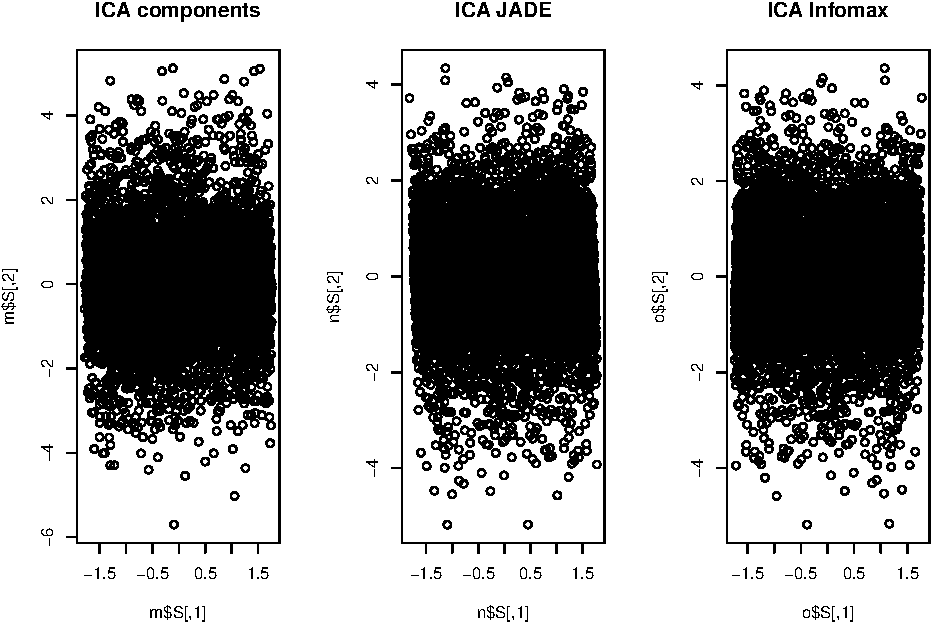
\includegraphics{ICAStatsComps_files/figure-latex/unnamed-chunk-10-1} \end{center}
  
  While JADE and Infomax at \(nc=2\) do not differ greatly from \(nc=4\),
  the fastICA plot appears more similar to the pre-processed data when the
  number of components is set at 4.
  
  \subsubsection{Congruence Coefficient of Source
  Signals}\label{congruence-coefficient-of-source-signals}
  
  \begin{verbatim}
     Method        Coeff
  1 fastICA 0.0018272806
  2    JADE 0.0032751124
  3 Infomax 0.0009626886
  \end{verbatim}
  
  For the CPP data, the congruence coefficient compares the this value
  between the observed data and generated source data, as the true \(S\)
  is not known like in the Random Uniform case. Thus, a lower value for
  our absolute max congruence coefficient should be optimal. Again,
  running the ICA methods on more than one dataset will provide more
  robust results.
  
  \section{Simulation}\label{simulation}
  
  Given the simplistic nature of both toy examples, a simulation can
  provide more robust insight into the effectiveness of ICA in extracting
  original source components.
  
  \subsection{Random Uniform Distribution
  Simulation}\label{random-uniform-distribution-simulation}
  
  Adding noise to the Random Uniform example will be done by generating a
  noise vector from a random exponential distribution with \(\lambda= 1\).
  This should inform how fastICA, JADE and Infomax perform when the Random
  Uniform data has been obscured further beyond the mixing matrix A.
  
  \begin{Shaded}
  \begin{Highlighting}[]
  \NormalTok{n <-}\StringTok{ }\DecValTok{1000}
  \KeywordTok{set.seed}\NormalTok{(}\DecValTok{10}\NormalTok{)}
  \NormalTok{sim_S <-}\StringTok{ }\ControlFlowTok{function}\NormalTok{(n,noise) \{ }
  \NormalTok{  U <-}\StringTok{ }\KeywordTok{runif}\NormalTok{(n, }\DecValTok{0}\NormalTok{,}\DecValTok{1}\NormalTok{)}
  \NormalTok{  samples <-}\StringTok{ }\KeywordTok{rep}\NormalTok{(}\DecValTok{0}\NormalTok{,n)}
  \CommentTok{# Add noise from a Random Exponential Distribution with lambda = 1}
  \NormalTok{  X <-}\StringTok{ }\KeywordTok{rexp}\NormalTok{(n,}\DecValTok{1}\NormalTok{) }
  \NormalTok{  S <-}\StringTok{ }\KeywordTok{runif}\NormalTok{(}\DecValTok{10000}\NormalTok{)}
    \ControlFlowTok{for}\NormalTok{(i }\ControlFlowTok{in} \DecValTok{1}\OperatorTok{:}\NormalTok{n) \{}
  \CommentTok{# Higher the noise value, the more we sample from noise vector}
      \ControlFlowTok{if}\NormalTok{(U[i]}\OperatorTok{<}\NormalTok{noise) \{ }
  \NormalTok{      samples[i] =}\StringTok{ }\NormalTok{X[i]}
  
  \NormalTok{    \}}\ControlFlowTok{else}\NormalTok{ \{}
  \NormalTok{      samples[i] =}\StringTok{ }\NormalTok{S[i]\}}
  
  \NormalTok{  \}}
  \NormalTok{    m.samples <-}\StringTok{ }\KeywordTok{matrix}\NormalTok{(samples,N,}\DecValTok{2}\NormalTok{,}\DataTypeTok{byrow=}\NormalTok{T)}
    \KeywordTok{return}\NormalTok{(m.samples)}
    
  \NormalTok{\}}
  \end{Highlighting}
  \end{Shaded}
  
  \begin{Shaded}
  \begin{Highlighting}[]
  \NormalTok{N <-}\StringTok{ }\DecValTok{1000}
  
  \CommentTok{# Create 3 empty vectors for each ICA algorithm }
  \NormalTok{itF <-}\StringTok{ }\KeywordTok{rep}\NormalTok{(}\OtherTok{NA}\NormalTok{,}\DecValTok{1}\NormalTok{,N) }
  \NormalTok{itJ <-}\StringTok{ }\KeywordTok{rep}\NormalTok{(}\OtherTok{NA}\NormalTok{,}\DecValTok{1}\NormalTok{,N)}
  \NormalTok{itM <-}\StringTok{ }\KeywordTok{rep}\NormalTok{(}\OtherTok{NA}\NormalTok{,}\DecValTok{1}\NormalTok{,N)}
  \NormalTok{JF <-}\StringTok{ }\KeywordTok{rep}\NormalTok{(}\OtherTok{NA}\NormalTok{, }\DecValTok{1}\NormalTok{,N)}
  \NormalTok{A <-}\StringTok{ }\KeywordTok{matrix}\NormalTok{(}\KeywordTok{c}\NormalTok{(}\DecValTok{1}\NormalTok{, }\DecValTok{1}\NormalTok{, }\OperatorTok{-}\DecValTok{1}\NormalTok{, }\DecValTok{3}\NormalTok{), }\DecValTok{2}\NormalTok{, }\DecValTok{2}\NormalTok{, }\DataTypeTok{byrow =} \OtherTok{TRUE}\NormalTok{)}
  
  \CommentTok{#Function to find colMax of the generated congruencey coefficients}
  
  \NormalTok{colMax <-}\StringTok{ }\ControlFlowTok{function}\NormalTok{(data) }\KeywordTok{sapply}\NormalTok{(data, max, }\DataTypeTok{na.rm =} \OtherTok{TRUE}\NormalTok{)[}\DecValTok{1}\NormalTok{] }
  
  \NormalTok{gen <-}\StringTok{ }\ControlFlowTok{function}\NormalTok{(N,S, noise)  \{ }
  \CommentTok{#Inputs: number of interations,amount of noise,}
  \CommentTok{# and source signal matrix }
    
    \ControlFlowTok{for}\NormalTok{ (i }\ControlFlowTok{in} \DecValTok{1}\OperatorTok{:}\NormalTok{N) \{}
  \NormalTok{    X[i] <-}\StringTok{ }\KeywordTok{sim_S}\NormalTok{(N,noise) }\OperatorTok\StringTok{ }\NormalTok{A }
  \NormalTok{    a <-}\StringTok{ }\KeywordTok{fastICA}\NormalTok{(X, }\DecValTok{2}\NormalTok{, }\DataTypeTok{alg.typ =} \StringTok{"parallel"}\NormalTok{, }\DataTypeTok{fun =} \StringTok{"logcosh"}\NormalTok{, }\DataTypeTok{alpha =} \DecValTok{1}\NormalTok{, }
                   \DataTypeTok{method =} \StringTok{"C"}\NormalTok{, }\DataTypeTok{row.norm =} \OtherTok{FALSE}\NormalTok{, }\DataTypeTok{maxit =} \DecValTok{200}\NormalTok{, }
                   \DataTypeTok{tol =} \FloatTok{0.0001}\NormalTok{, }\DataTypeTok{verbose =} \OtherTok{TRUE}\NormalTok{)}
  \NormalTok{    b<-}\StringTok{ }\KeywordTok{icajade}\NormalTok{(X,}\DecValTok{2}\NormalTok{,}\DataTypeTok{center=}\OtherTok{TRUE}\NormalTok{,}\DataTypeTok{maxit=}\DecValTok{200}\NormalTok{,}\DataTypeTok{tol=}\FloatTok{0.0001}\NormalTok{)}
      
  \NormalTok{    c<-}\StringTok{ }\KeywordTok{icaimax}\NormalTok{(X,}\DataTypeTok{nc=}\DecValTok{2}\NormalTok{,}\DataTypeTok{center=}\OtherTok{TRUE}\NormalTok{,}\DataTypeTok{maxit=}\DecValTok{200}\NormalTok{,}\DataTypeTok{tol=}\FloatTok{0.0001}\NormalTok{,}
                  \DataTypeTok{alg=}\StringTok{"newton"}\NormalTok{,}\DataTypeTok{fun=}\StringTok{"log"}\NormalTok{)}
      
  \CommentTok{# Store a Absolute Maximum Congruence Coefficient for }
  \CommentTok{# each N iteration of the ICA model}
  \NormalTok{    itF[i] <-}\StringTok{ }\KeywordTok{colMax}\NormalTok{(}\KeywordTok{abs}\NormalTok{(}\KeywordTok{congru}\NormalTok{(S,a}\OperatorTok{$}\NormalTok{S)))}
  \NormalTok{    itJ[i] <-}\StringTok{ }\KeywordTok{colMax}\NormalTok{(}\KeywordTok{abs}\NormalTok{(}\KeywordTok{congru}\NormalTok{(S,b}\OperatorTok{$}\NormalTok{S)))}
  \NormalTok{    itM[i] <-}\StringTok{ }\KeywordTok{colMax}\NormalTok{(}\KeywordTok{abs}\NormalTok{(}\KeywordTok{congru}\NormalTok{(S,c}\OperatorTok{$}\NormalTok{S)))}
      
  \CommentTok{# This compares Absolute Maximum Congruence Coefficient between fastICA and JADE}
      
  \NormalTok{    JF[i] <-}\StringTok{ }\KeywordTok{colMax}\NormalTok{(}\KeywordTok{abs}\NormalTok{(}\KeywordTok{congru}\NormalTok{(a}\OperatorTok{$}\NormalTok{S,b}\OperatorTok{$}\NormalTok{S)))}
  
  \NormalTok{  \}}
    \CommentTok{# Return a list of values from each method}
    \KeywordTok{return}\NormalTok{(}\KeywordTok{list}\NormalTok{(itF,itJ,itM,JF))}
  \NormalTok{\}}
  
  \CommentTok{# Generate Coefficients for N datasets at multiple noise levels}
  
  \NormalTok{I1 <-}\StringTok{ }\KeywordTok{gen}\NormalTok{(N,S,}\FloatTok{0.05}\NormalTok{) }\CommentTok{# Noise = 0.05  Norm values }
  \NormalTok{I2 <-}\StringTok{ }\KeywordTok{gen}\NormalTok{(N,S,}\FloatTok{0.10}\NormalTok{) }\CommentTok{# Noise = 0.10 Norm values}
  \NormalTok{I3 <-}\StringTok{ }\KeywordTok{gen}\NormalTok{(N,S,}\FloatTok{0.15}\NormalTok{) }\CommentTok{# Noise = 0.15 Norm values}
  \NormalTok{NoNoise <-}\StringTok{ }\KeywordTok{gen}\NormalTok{(N,S,}\DecValTok{0}\NormalTok{)  }\CommentTok{# Noise = 0 / No Noise}
  \end{Highlighting}
  \end{Shaded}
  
  \subsection{Noise = 0 Results}\label{noise-0-results}
  
  \begin{verbatim}
      column    n      mean         sd    median   trimmed        mad
  1  fastICA 1000 0.1638213 0.13109493 0.1375945 0.1484611 0.11741881
  2     JADE 1000 0.1024091 0.04922798 0.1167199 0.1073506 0.05138732
  3  Infomax 1000 0.1003643 0.05153871 0.1155706 0.1050809 0.05374063
  4 JadeFast 1000 0.5240766 0.47524293 0.6889716 0.5287862 0.46111155
             min       max     range        skew   kurtosis          se
  1 1.660327e-04 0.4877045 0.4875384  0.94597205 -0.1645861 0.004145586
  2 1.049017e-03 0.1526784 0.1516294 -0.55175316 -1.1498735 0.001556725
  3 9.359263e-06 0.1535549 0.1535456 -0.48932480 -1.2989490 0.001629797
  4 4.176865e-03 0.9999916 0.9958147 -0.02324014 -1.9847584 0.015028501
  \end{verbatim}
  
  The expectation for the value of Absolute Maximum Congruence Coefficient
  for the noiseless model was for it to be high (eg. close to 1, the
  highest value) since the true S and the generated S by the algorithms
  should be similar. However, this was not the case, particularly for JADE
  and Infomax, as their means were below \(0.10\) with SD of around
  \(0.044\). fastICA's mean was larger, but the SD was high at around
  \(0.125\).
  
  Thus, the Absolute Maximum Congruence Coefficient between fastICA and
  JADE was also calculated for a sanity check, and was found to be close
  to \(0.51\) but also had a high standard deviation. Interestingly, the
  median was actually close 1 at 0.9988695, suggesting that the algorithms
  performed relatively similarly.
  
  \subsection{Noise = 0.05 Results}\label{noise-0.05-results}
  
  \begin{verbatim}
      column    n      mean         sd    median   trimmed        mad
  1  fastICA 1000 0.1489319 0.09964877 0.1346393 0.1376030 0.04651286
  2     JADE 1000 0.1285576 0.02007665 0.1330783 0.1300112 0.02079712
  3  Infomax 1000 0.1243085 0.02718760 0.1318008 0.1279910 0.02393317
  4 JadeFast 1000 0.5399478 0.48143559 0.9563555 0.5495371 0.06470635
             min       max     range       skew  kurtosis           se
  1 3.334330e-04 0.4877898 0.4874563  1.1591724  1.246994 0.0031511709
  2 3.785129e-03 0.1555764 0.1517913 -2.1263283 10.416212 0.0006348793
  3 4.905307e-03 0.1521648 0.1472594 -1.9849818  5.459700 0.0008597475
  4 5.344373e-05 1.0000000 0.9999466 -0.1250572 -1.957931 0.0152243302
  \end{verbatim}
  
  Unsurprisingly, the results when a small amount of noise was added to
  our data was essentially the same as for the NoNoise simulation.
  However, it seems strange that the JADE and Infomax algorithms behaved
  more similar to each other for this model with some additional noise.
  
  Again, comparing fastICA and JADE as an alternative approach, they
  appeared to perform about equally on this noisier model with a mean of
  \(0.547\) and a median of \(0.924\).
  
  \subsection{Noise = 0.10 Results}\label{noise-0.10-results}
  
  \begin{verbatim}
      column    n      mean         sd    median   trimmed        mad
  1  fastICA 1000 0.1615841 0.11899359 0.1408028 0.1471446 0.06225168
  2     JADE 1000 0.1295651 0.03908884 0.1446667 0.1396517 0.01037763
  3  Infomax 1000 0.1188921 0.04516841 0.1380394 0.1289802 0.01988052
  4 JadeFast 1000 0.5257030 0.46904189 0.3589025 0.5301044 0.52473593
             min       max     range        skew   kurtosis          se
  1 2.655194e-04 0.4877920 0.4875265  1.06081461  0.6014137 0.003762908
  2 2.422218e-05 0.1529682 0.1529439 -2.28344998  4.1430261 0.001236098
  3 1.105514e-03 0.1522820 0.1511765 -1.73089978  1.6937317 0.001428351
  4 3.400405e-03 0.9999930 0.9965926 -0.01229774 -1.9723536 0.014832407
  \end{verbatim}
  
  Both JADE and Infomax ``improved'' at the 0.10 noise level, and fastICA
  variability fell marginally.The fastICA JADE did not demonstrate the
  same success as the median value is only \(0.407\), suggesting increased
  dissimilarity in results from the two methods.
  
  \subsection{Noise = 0.15 Results}\label{noise-0.15-results}
  
  \begin{verbatim}
      column    n      mean         sd    median   trimmed         mad
  1  fastICA 1000 0.1517650 0.08694443 0.1464803 0.1454231 0.025503600
  2     JADE 1000 0.1582890 0.01587534 0.1562030 0.1583514 0.007266911
  3  Infomax 1000 0.1469350 0.01670913 0.1486793 0.1487019 0.002560352
  4 JadeFast 1000 0.5447331 0.45285642 0.9042250 0.5489777 0.141995965
             min       max     range        skew  kurtosis           se
  1 0.0002573546 0.4876775 0.4874202  0.93470598  1.746629 0.0027494243
  2 0.0062724214 0.1889853 0.1827129 -5.86205706 54.876948 0.0005020225
  3 0.0071266111 0.1660601 0.1589335 -7.19399671 53.212491 0.0005283891
  4 0.0044797527 1.0000000 0.9955202 -0.02841594 -1.981007 0.0143205773
  \end{verbatim}
  
  Oddly enough, all three algorithms performed their best (largest mean
  value) on the 0.15 noise model, perhaps this indicates a need to run
  more iterations in order to recover more of the uniform distributions.
  Additionally, the random uniform may just have a high level of
  randomness for each dataset that does not allow the Absolute Maximum
  Congruence Coefficient to perform well.
  
  Again, the JADE and fastICA comparison demonstrated that the performed
  roughly the same under these conditions.
  
  \section{CPP Simulation:}\label{cpp-simulation}
  
  \subsection{Adding noise from Random
  Uniform}\label{adding-noise-from-random-uniform}
  
  \begin{Shaded}
  \begin{Highlighting}[]
  \NormalTok{x <-}\StringTok{ }\KeywordTok{data}\NormalTok{(CPPdata)}
  \KeywordTok{set.seed}\NormalTok{(}\DecValTok{40}\NormalTok{)}
  \NormalTok{dat <-}\StringTok{ }\NormalTok{CPPdata[}\KeywordTok{sample}\NormalTok{(}\DecValTok{10000}\NormalTok{),]}
  \NormalTok{mix <-}\KeywordTok{matrix}\NormalTok{(}\KeywordTok{runif}\NormalTok{(}\DecValTok{10000}\NormalTok{),}\DecValTok{10000}\NormalTok{,}\DecValTok{4}\NormalTok{)}
  \NormalTok{N <-}\StringTok{ }\DecValTok{10000}
  \NormalTok{t <-}\StringTok{ }\KeywordTok{rep}\NormalTok{(}\OtherTok{NA}\NormalTok{,}\DecValTok{4}\NormalTok{)}
  
  \NormalTok{sim_CPP <-}\StringTok{ }\ControlFlowTok{function}\NormalTok{(N,noise) \{}
  \NormalTok{  samples <-}\StringTok{ }\KeywordTok{rep}\NormalTok{(}\DecValTok{0}\NormalTok{,N)}
  \NormalTok{  t <-}\StringTok{ }\DecValTok{1}\OperatorTok{:}\DecValTok{4}
  \NormalTok{  U <-}\StringTok{ }\KeywordTok{runif}\NormalTok{(N,}\DecValTok{0}\NormalTok{,}\DecValTok{1}\NormalTok{)}
    \ControlFlowTok{for}\NormalTok{(i }\ControlFlowTok{in} \DecValTok{1}\OperatorTok{:}\NormalTok{N) \{}
        \ControlFlowTok{if}\NormalTok{(U[i]}\OperatorTok{<}\NormalTok{noise) \{}
  \NormalTok{          samples[i] =}\StringTok{ }\KeywordTok{runif}\NormalTok{(N,}\DecValTok{0}\NormalTok{,}\DecValTok{10}\NormalTok{)[i]}
  
  \NormalTok{      \}}\ControlFlowTok{else}\NormalTok{ \{}
  \NormalTok{          samples[i] =}\StringTok{ }\NormalTok{CPPdata[}\KeywordTok{sample}\NormalTok{(N),}\KeywordTok{sample}\NormalTok{(t)[}\DecValTok{1}\NormalTok{]]}
  \NormalTok{      \}}
  \NormalTok{  \}}
  \NormalTok{    m.samples <-}\StringTok{ }\KeywordTok{matrix}\NormalTok{(samples,N,}\DecValTok{4}\NormalTok{,}\DataTypeTok{byrow=}\NormalTok{T)}
    \KeywordTok{return}\NormalTok{(m.samples)}
  \NormalTok{\}}
  \end{Highlighting}
  \end{Shaded}
  
  \begin{Shaded}
  \begin{Highlighting}[]
  \NormalTok{N <-}\StringTok{ }\DecValTok{500}
  \NormalTok{C_S <-}\StringTok{ }\KeywordTok{as.matrix}\NormalTok{(dat)[}\KeywordTok{sample}\NormalTok{(N),]}
  \NormalTok{itCF <-}\StringTok{ }\KeywordTok{rep}\NormalTok{(}\OtherTok{NA}\NormalTok{,}\DecValTok{1}\NormalTok{,N)}
  \NormalTok{itCJ <-}\StringTok{ }\KeywordTok{rep}\NormalTok{(}\OtherTok{NA}\NormalTok{,}\DecValTok{1}\NormalTok{,N)}
  \NormalTok{itCM <-}\StringTok{ }\KeywordTok{rep}\NormalTok{(}\OtherTok{NA}\NormalTok{,}\DecValTok{1}\NormalTok{,N)}
  \NormalTok{JF2 <-}\StringTok{ }\KeywordTok{rep}\NormalTok{(}\OtherTok{NA}\NormalTok{,}\DecValTok{1}\NormalTok{,N)}
  
  \NormalTok{gen_CPP <-}\StringTok{ }\ControlFlowTok{function}\NormalTok{(N,S, noise)  \{}
    \ControlFlowTok{for}\NormalTok{ (i }\ControlFlowTok{in} \DecValTok{1}\OperatorTok{:}\NormalTok{N) \{}
  \NormalTok{    X <-}\StringTok{ }\KeywordTok{sim_CPP}\NormalTok{(N,noise)}
  \NormalTok{    m <-}\StringTok{ }\KeywordTok{fastICA}\NormalTok{(X,}\DecValTok{2}\NormalTok{,}\DataTypeTok{alg.typ =} \StringTok{"parallel"}\NormalTok{, }\DataTypeTok{fun =} \StringTok{"logcosh"}\NormalTok{, }\DataTypeTok{alpha =} \DecValTok{1}\NormalTok{, }
               \DataTypeTok{method =} \StringTok{"C"}\NormalTok{, }\DataTypeTok{row.norm =} \OtherTok{FALSE}\NormalTok{, }\DataTypeTok{maxit =} \DecValTok{200}\NormalTok{, }
               \DataTypeTok{tol =} \FloatTok{0.0001}\NormalTok{, }\DataTypeTok{verbose =} \OtherTok{TRUE}\NormalTok{)}
  \NormalTok{    n <-}\StringTok{ }\KeywordTok{icajade}\NormalTok{(X,}\DecValTok{4}\NormalTok{,}\DataTypeTok{center=}\OtherTok{TRUE}\NormalTok{,}\DataTypeTok{maxit=}\DecValTok{200}\NormalTok{,}\DataTypeTok{tol=}\FloatTok{0.0001}\NormalTok{)}
  
  \NormalTok{    o <-}\StringTok{ }\KeywordTok{icaimax}\NormalTok{(X,}\DataTypeTok{nc=}\DecValTok{4}\NormalTok{,}\DataTypeTok{center=}\OtherTok{TRUE}\NormalTok{,}\DataTypeTok{maxit=}\DecValTok{200}\NormalTok{,}\DataTypeTok{tol=}\FloatTok{0.0001}\NormalTok{,}
                   \DataTypeTok{alg=}\StringTok{"newton"}\NormalTok{,}\DataTypeTok{fun=}\StringTok{"log"}\NormalTok{)}
  
  \NormalTok{    itCF[i] <-}\StringTok{ }\KeywordTok{colMax}\NormalTok{(}\KeywordTok{abs}\NormalTok{(}\KeywordTok{congru}\NormalTok{(C_S,m}\OperatorTok{$}\NormalTok{S)))}
  \NormalTok{    itCJ[i] <-}\StringTok{ }\KeywordTok{colMax}\NormalTok{(}\KeywordTok{abs}\NormalTok{(}\KeywordTok{congru}\NormalTok{(C_S,n}\OperatorTok{$}\NormalTok{S)))}
  \NormalTok{    itCM[i] <-}\StringTok{ }\KeywordTok{colMax}\NormalTok{(}\KeywordTok{abs}\NormalTok{(}\KeywordTok{congru}\NormalTok{(C_S,o}\OperatorTok{$}\NormalTok{S)))}
  \NormalTok{    JF2[i] <-}\StringTok{ }\KeywordTok{colMax}\NormalTok{(}\KeywordTok{abs}\NormalTok{(}\KeywordTok{congru}\NormalTok{(n}\OperatorTok{$}\NormalTok{S,m}\OperatorTok{$}\NormalTok{S)))}
  
  \NormalTok{  \}}
    \KeywordTok{return}\NormalTok{(}\KeywordTok{list}\NormalTok{(itCF,itCJ,itCM,JF2))}
  \NormalTok{\}}
  \NormalTok{IC1 <-}\StringTok{ }\KeywordTok{gen_CPP}\NormalTok{(N,C_S,}\FloatTok{0.05}\NormalTok{) }\CommentTok{# Noise = 0.05  }
  \NormalTok{IC2 <-}\StringTok{ }\KeywordTok{gen_CPP}\NormalTok{(N,C_S,}\FloatTok{0.10}\NormalTok{) }\CommentTok{# Noise = 0.10 }
  \NormalTok{IC3 <-}\StringTok{ }\KeywordTok{gen_CPP}\NormalTok{(N,C_S,}\FloatTok{0.15}\NormalTok{)  }\CommentTok{# Noise = 0.15 }
  \NormalTok{NN2 <-}\StringTok{ }\KeywordTok{gen_CPP}\NormalTok{(N,C_S,}\DecValTok{0}\NormalTok{)}
  \end{Highlighting}
  \end{Shaded}
  
  \subsection{Noise = 0 Results}\label{noise-0-results-1}
  
  \begin{verbatim}
      column   n        mean          sd      median     trimmed         mad
  1  fastICA 500 0.005989154 0.004695226 0.004878922 0.005444689 0.004256639
  2     JADE 500 0.005697663 0.004477445 0.004750534 0.005169665 0.004408381
  3  Infomax 500 0.005716690 0.004693025 0.004435234 0.005149401 0.004381271
  4 JadeFast 500 0.505330809 0.356041955 0.539719093 0.507151751 0.536848127
             min        max      range        skew   kurtosis           se
  1 3.618137e-05 0.02605655 0.02602036  1.05563779  0.8880875 0.0002099769
  2 2.355080e-05 0.02295155 0.02292799  0.97077381  0.5105231 0.0002002374
  3 6.902722e-06 0.02250676 0.02249986  0.99808237  0.4336876 0.0002098785
  4 1.624218e-03 0.99955303 0.99792881 -0.04310171 -1.6485584 0.0159226803
  \end{verbatim}
  
  The comparison by Absolute Maximum Congruence Coefficient for the CPP
  proves slightly more difficult since the true S is not known (comparison
  of congruence here is done between the data and generated S not known S
  as mentioned earlier). Regardless, each algorithm performed very
  similarly (means within 0.0003 of each other) and had low standard
  deviation, thus the noiseless model seems to be relatively indifferent
  between the models. The Jade and FastICA test resulted in a mean of
  \(0.511\), suggesting relative similarity in the two methods.
  
  \subsection{Noise = 0.05 Results}\label{noise-0.05-results-1}
  
  \begin{verbatim}
      column   n        mean          sd      median     trimmed         mad
  1  fastICA 500 0.005839718 0.004641555 0.004927834 0.005268833 0.004494524
  2     JADE 500 0.005781619 0.004465908 0.004901945 0.005283814 0.004393377
  3  Infomax 500 0.005776980 0.004360168 0.004914277 0.005325630 0.004420861
  4 JadeFast 500 0.536839683 0.325429353 0.591683862 0.545462039 0.440532969
             min        max      range       skew   kurtosis           se
  1 1.914060e-05 0.02685490 0.02683576  1.0472508  0.9069099 0.0002075766
  2 5.288971e-05 0.02347204 0.02341915  1.0056448  0.7555682 0.0001997215
  3 2.482226e-06 0.02175965 0.02175717  0.8992272  0.4414992 0.0001949926
  4 1.216242e-03 0.99456224 0.99334599 -0.1838815 -1.4800576 0.0145536431
  \end{verbatim}
  
  Results for the lowest level of noise are even closer than in the
  noiseless model. Jade and FastICA comparison performs slightly better in
  this case, suggesting closer performance.
  
  \subsection{Noise = 0.10 Results}\label{noise-0.10-results-1}
  
  \begin{verbatim}
      column   n        mean          sd      median     trimmed         mad
  1  fastICA 500 0.005925766 0.004351024 0.005267391 0.005483064 0.004477307
  2     JADE 500 0.005902257 0.004513415 0.004923009 0.005409258 0.004317833
  3  Infomax 500 0.005940126 0.004409482 0.005133846 0.005482307 0.004196482
  4 JadeFast 500 0.551310470 0.313737413 0.622876286 0.564327966 0.379089057
             min        max      range       skew   kurtosis           se
  1 4.174936e-06 0.02147595 0.02147177  0.8480802  0.2542811 0.0001945837
  2 1.530885e-05 0.02659126 0.02657596  1.0098493  0.8982511 0.0002018460
  3 1.674796e-06 0.02677447 0.02677279  0.9745771  0.7996612 0.0001971980
  4 1.357246e-03 0.99994625 0.99858900 -0.3430005 -1.2804338 0.0140307636
  \end{verbatim}
  
  Once again, all 3 algorithms produce almost identical means. Jade to
  FastICA comparison is similar to prior comparisons.
  
  \subsection{Noise = 0.15 Results}\label{noise-0.15-results-1}
  
  \begin{verbatim}
      column   n        mean          sd      median     trimmed         mad
  1  fastICA 500 0.005923584 0.004366387 0.005129439 0.005461611 0.004364728
  2     JADE 500 0.006243437 0.004499542 0.005326893 0.005755261 0.004323296
  3  Infomax 500 0.006003017 0.004569875 0.004994865 0.005499254 0.004515031
  4 JadeFast 500 0.537741988 0.313622884 0.575066472 0.547251464 0.418546575
             min        max      range       skew   kurtosis           se
  1 7.304603e-06 0.02073405 0.02072675  0.8870981  0.3354806 0.0001952708
  2 8.044330e-06 0.02356652 0.02355847  0.9295177  0.4837393 0.0002012256
  3 2.844015e-05 0.02439330 0.02436486  0.9784172  0.6836353 0.0002043710
  4 2.052682e-05 0.98760350 0.98758297 -0.2043053 -1.3882923 0.0140256418
  \end{verbatim}
  
  The highest Noise threshold behaved most similarly to the noiseless, in
  terms of slightly more variability between algorithms. The Jade to
  FastICA comparison behaved similarly to the Noise = 0.05 case.
  
  \subsection{Method Effectiveness}\label{method-effectiveness}
  
  In conclusion, differentiating between the various ICA model algorithms
  may not be particular important in analysis aside from wanting a use a
  particular non-Gaussian estimator or because of the need to control a
  certain parameter within the function. Notably, JADE has fewer inputs
  than Infomax or fastICA, thus has more limited flexibility. For the
  purposes of the rest of this paper, only the fastICA algorithm will be
  utilized.
  
  \chapter{Computation and Application to
  Dataset}\label{computation-and-application-to-dataset}
  
  \section{Dataset 1: Walmart Store Data from
  Kaggle}\label{dataset-1-walmart-store-data-from-kaggle}
  
  From a 2014 Kaggle competition with a goal of forecasting Walmart Sales,
  the Walmart Store dataset provides information on sales for \(n=45\)
  located in different regions of the United States. Each store has Weekly
  Sales data from \(2010-02-05\) to \(2012-11-01\), information by
  department and a binary IsHoliday variable. Evidently, this data has
  fairly limited number of predictors but was one of few available retail
  datasets, thus was used as a warm up application before applying to a
  larger dataset.
  
  (Kaggle/Walmart, 2017)
  
  \subsection{Prior Analysis : Kimmo Kiviluoto and Erkki
  Oja}\label{prior-analysis-kimmo-kiviluoto-and-erkki-oja}
  
  In 1998, Kiviluoto and Erkki Oja used ICA on parallel Financial Time
  Series from a retail chain of 40 stores. They claim in their paper
  \textit{Independent Component Analysis for Parallel Financial Time Series}
  that by removing the fundamental factors of the data, they were able to
  see the impact of management decisions of a particular store more
  clearly. (pg. 2, {\textbf{???}})
  
  With the Walmart store data, an attempt to show a similar, interesting
  result using retail data will be made. However, this will look at Weekly
  Sales not Cash-flow data, which will probably not generate as robust
  results since cash-flow provides more information about financial
  activities of a store than just sales.
  
  \subsection{Exploration}\label{exploration}
  
  \section{FastICA Application}\label{fastica-application}
  
  \begin{Shaded}
  \begin{Highlighting}[]
  \CommentTok{# Set nc= 3 based on dimensions}
  \NormalTok{a <-}\KeywordTok{fastICA}\NormalTok{(w2,}\DecValTok{3}\NormalTok{, }\DataTypeTok{alg.typ=}\StringTok{"parallel"}\NormalTok{,}\DataTypeTok{fun=} \StringTok{"logcosh"}\NormalTok{,}\DataTypeTok{row.norm=}\OtherTok{FALSE}\NormalTok{,}\DataTypeTok{maxit=}\DecValTok{5}\NormalTok{,}\DataTypeTok{tol=} \FloatTok{0.0001}\NormalTok{,}\DataTypeTok{verbose=}\OtherTok{TRUE}\NormalTok{)}
  \KeywordTok{par}\NormalTok{(}\DataTypeTok{mfrow =} \KeywordTok{c}\NormalTok{(}\DecValTok{1}\NormalTok{, }\DecValTok{3}\NormalTok{))}
  \KeywordTok{plot}\NormalTok{(a}\OperatorTok{$}\NormalTok{X, }\DataTypeTok{main =} \StringTok{"Pre-processed data"}\NormalTok{)}
  \KeywordTok{plot}\NormalTok{(a}\OperatorTok{$}\NormalTok{X }\OperatorTok\StringTok{ }\NormalTok{a}\OperatorTok{$}\NormalTok{K, }\DataTypeTok{main =} \StringTok{"PCA components"}\NormalTok{ )}
  \KeywordTok{plot}\NormalTok{(a}\OperatorTok{$}\NormalTok{S, }\DataTypeTok{main =} \StringTok{"fastICA components"}\NormalTok{)  }
  \end{Highlighting}
  \end{Shaded}
  
  \begin{center}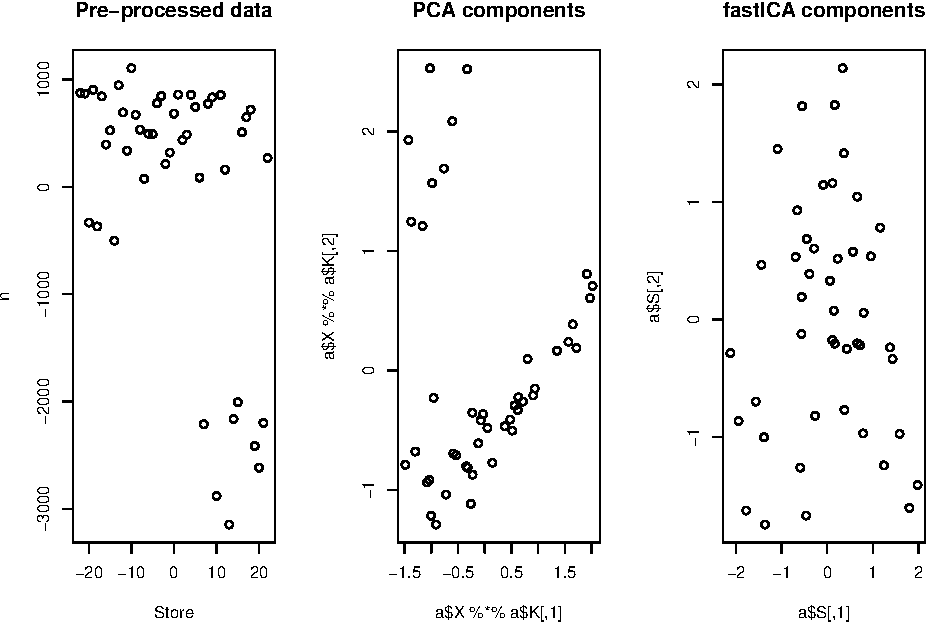
\includegraphics{ICAStatsComps_files/figure-latex/unnamed-chunk-25-1} \end{center}
  
  From these plots, there appears to be some clustering uncovered by the
  fastICA algorithm. One possibility is that the cluster of 8 stores at
  towards the top represents the most productive in terms of sales but
  this could just be random noise. In general,the dataset appears to be
  too small in terms of both dimensions and observations to come to any
  explicit conclusions about underlying influences of Weekly Sales and top
  performing stores.
  
  \subsection{Dataset 2: Sample Superstore
  data}\label{dataset-2-sample-superstore-data}
  
  The Superstore Sample data appears in the December Tableau User Group
  presentation.
  
  Since this data has higher dimensionality and more variety of variables,
  the ICA model should be more effective here. Unlike with the prior
  simulations, only the fastICA algorithm will be used. (Tableau, 2017)
  
  Note: Geographic locations have been altered to include Canadian
  locations numerically (provinces / regions). \newline
  
  \subsection{Select Variables of
  Interest}\label{select-variables-of-interest}
  
  \subsubsection{Sample of Variables}\label{sample-of-variables}
  
  \begin{verbatim}
  # A tibble: 21 x 1
                  x
              <chr>
   1         Row ID
   2       Order ID
   3     Order Date
   4 Order Priority
   5 Order Quantity
   6          Sales
   7       Discount
   8      Ship Mode
   9         Profit
  10     Unit Price
  # ... with 11 more rows
  \end{verbatim}
  
  \subsubsection{By Province}\label{by-province}
  
  \begin{Shaded}
  \begin{Highlighting}[]
  \NormalTok{s <-}\StringTok{ }\NormalTok{store }\OperatorTok\StringTok{ }
  \StringTok{  }\KeywordTok{select}\NormalTok{(}\StringTok{`}\DataTypeTok{Order ID}\StringTok{`}\NormalTok{,}\StringTok{`}\DataTypeTok{Row ID}\StringTok{`}\NormalTok{,}\StringTok{`}\DataTypeTok{Order Date}\StringTok{`}\NormalTok{,}\StringTok{`}\DataTypeTok{Order Quantity}\StringTok{`}\NormalTok{,Sales, Discount, Profit,}\StringTok{`}\DataTypeTok{Unit Price}\StringTok{`}\NormalTok{, }\StringTok{`}\DataTypeTok{Shipping Cost}\StringTok{`}\NormalTok{,Province) }\OperatorTok
  \StringTok{  }\KeywordTok{group_by}\NormalTok{(Province) }\OperatorTok\StringTok{ }\KeywordTok{summarise}\NormalTok{(}\DataTypeTok{n =} \KeywordTok{n}\NormalTok{(),}
      \DataTypeTok{Order_Q =} \KeywordTok{sum}\NormalTok{(}\StringTok{`}\DataTypeTok{Order Quantity}\StringTok{`}\NormalTok{),}
      \DataTypeTok{Sales =} \KeywordTok{sum}\NormalTok{(Sales),}
      \DataTypeTok{Discount =} \KeywordTok{sum}\NormalTok{(Discount),}
      \DataTypeTok{Profit =} \KeywordTok{sum}\NormalTok{(Profit),}
      \DataTypeTok{U_Price =} \KeywordTok{sum}\NormalTok{(}\StringTok{`}\DataTypeTok{Unit Price}\StringTok{`}\NormalTok{),}
      \DataTypeTok{Ship_C =} \KeywordTok{sum}\NormalTok{(}\StringTok{`}\DataTypeTok{Shipping Cost}\StringTok{`}\NormalTok{))}
  
  \NormalTok{x <-}\StringTok{ }\NormalTok{s[,}\OperatorTok{-}\DecValTok{1}\NormalTok{] }\CommentTok{# Remove Province variables to fit ICA model (non-numeric)}
  \end{Highlighting}
  \end{Shaded}
  
  \begin{Shaded}
  \begin{Highlighting}[]
  \NormalTok{t <-}\StringTok{ }\KeywordTok{fastICA}\NormalTok{(x,}\DecValTok{4}\NormalTok{, }\DataTypeTok{alg.typ=}\StringTok{"parallel"}\NormalTok{,}\DataTypeTok{fun=} \StringTok{"logcosh"}\NormalTok{,}\DataTypeTok{row.norm=}\OtherTok{FALSE}\NormalTok{,}\DataTypeTok{maxit=}\DecValTok{5}\NormalTok{,}\DataTypeTok{tol=} \FloatTok{0.0001}\NormalTok{,}\DataTypeTok{verbose=}\OtherTok{TRUE}\NormalTok{)}
  \end{Highlighting}
  \end{Shaded}
  
  \begin{Shaded}
  \begin{Highlighting}[]
  \KeywordTok{par}\NormalTok{(}\DataTypeTok{mfrow =} \KeywordTok{c}\NormalTok{(}\DecValTok{1}\NormalTok{, }\DecValTok{3}\NormalTok{))}
  \KeywordTok{plot}\NormalTok{(t}\OperatorTok{$}\NormalTok{X, }\DataTypeTok{main =} \StringTok{"Pre-processed data"}\NormalTok{)}
  \KeywordTok{plot}\NormalTok{(t}\OperatorTok{$}\NormalTok{X }\OperatorTok\StringTok{ }\NormalTok{t}\OperatorTok{$}\NormalTok{K, }\DataTypeTok{main =} \StringTok{"PCA components"}\NormalTok{ )}
  \KeywordTok{plot}\NormalTok{(t}\OperatorTok{$}\NormalTok{S, }\DataTypeTok{main =} \StringTok{"ICA components"}\NormalTok{)  }
  \end{Highlighting}
  \end{Shaded}
  
  \begin{center}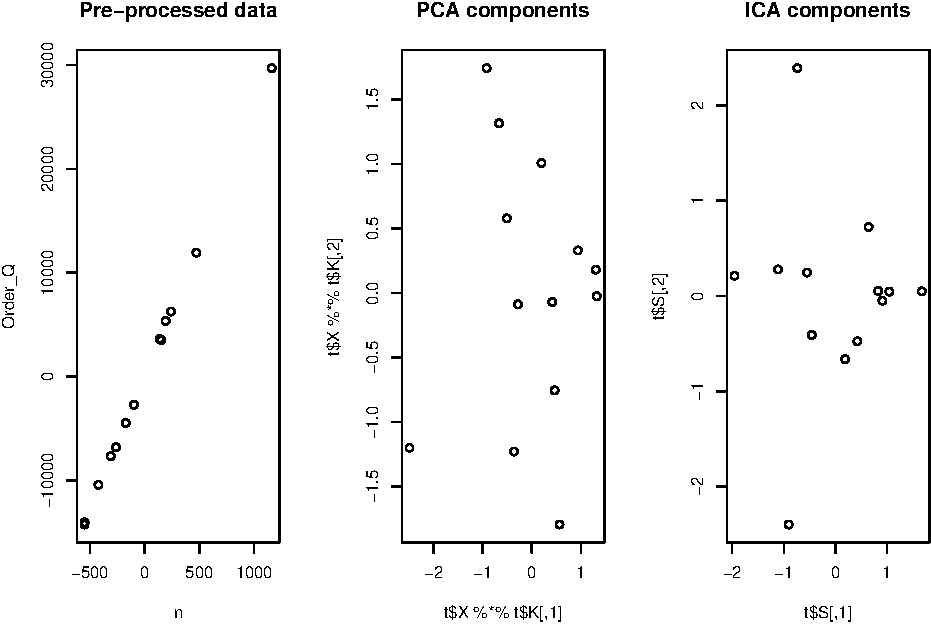
\includegraphics{ICAStatsComps_files/figure-latex/unnamed-chunk-30-1} \end{center}
  
  Looking at the superstore data by Province, some limited clustering
  exists that could potentially indicate nuances in store performance by
  Province or more volume of orders. Unfortunately, this view does not
  seem to be robust enough for any substantial conclusions.
  
  \subsubsection{By Order ID}\label{by-order-id}
  
  \begin{Shaded}
  \begin{Highlighting}[]
  \NormalTok{z <-}\StringTok{ }\NormalTok{store }\OperatorTok\StringTok{ }
  \StringTok{  }\KeywordTok{select}\NormalTok{(}\StringTok{`}\DataTypeTok{Order ID}\StringTok{`}\NormalTok{,}\StringTok{`}\DataTypeTok{Row ID}\StringTok{`}\NormalTok{,}\StringTok{`}\DataTypeTok{Order Date}\StringTok{`}\NormalTok{,}\StringTok{`}\DataTypeTok{Order Quantity}\StringTok{`}\NormalTok{,Sales, Discount, Profit,}\StringTok{`}\DataTypeTok{Unit Price}\StringTok{`}\NormalTok{, }\StringTok{`}\DataTypeTok{Shipping Cost}\StringTok{`}\NormalTok{,Province) }\OperatorTok
  \StringTok{  }\KeywordTok{group_by}\NormalTok{(}\StringTok{`}\DataTypeTok{Order ID}\StringTok{`}\NormalTok{) }\OperatorTok\StringTok{ }\KeywordTok{summarise}\NormalTok{(}
    \DataTypeTok{n =} \KeywordTok{n}\NormalTok{(),}
      \DataTypeTok{Order_Q =} \KeywordTok{sum}\NormalTok{(}\StringTok{`}\DataTypeTok{Order Quantity}\StringTok{`}\NormalTok{),}
      \DataTypeTok{Sales =} \KeywordTok{sum}\NormalTok{(Sales),}
      \DataTypeTok{Discount =} \KeywordTok{sum}\NormalTok{(Discount),}
      \DataTypeTok{Profit =} \KeywordTok{sum}\NormalTok{(Profit),}
      \DataTypeTok{U_Price =} \KeywordTok{sum}\NormalTok{(}\StringTok{`}\DataTypeTok{Unit Price}\StringTok{`}\NormalTok{),}
      \DataTypeTok{Ship_C =} \KeywordTok{sum}\NormalTok{(}\StringTok{`}\DataTypeTok{Shipping Cost}\StringTok{`}\NormalTok{))}
  \NormalTok{z1 <-}\StringTok{ }\NormalTok{z[}\KeywordTok{sample}\NormalTok{(}\DecValTok{1000}\NormalTok{),] }\CommentTok{#take sub sample}
  \end{Highlighting}
  \end{Shaded}
  
  \begin{Shaded}
  \begin{Highlighting}[]
  \NormalTok{test <-}\StringTok{ }\KeywordTok{fastICA}\NormalTok{(z1,}\DecValTok{8}\NormalTok{, }\DataTypeTok{alg.typ=}\StringTok{"parallel"}\NormalTok{,}\DataTypeTok{fun=} \StringTok{"logcosh"}\NormalTok{,}\DataTypeTok{row.norm=}\OtherTok{FALSE}\NormalTok{,}\DataTypeTok{maxit=}\DecValTok{5}\NormalTok{,}\DataTypeTok{tol=} \FloatTok{0.0001}\NormalTok{,}\DataTypeTok{verbose=}\OtherTok{TRUE}\NormalTok{)}
  \KeywordTok{par}\NormalTok{(}\DataTypeTok{mfrow =} \KeywordTok{c}\NormalTok{(}\DecValTok{1}\NormalTok{, }\DecValTok{3}\NormalTok{))}
  \KeywordTok{plot}\NormalTok{(test}\OperatorTok{$}\NormalTok{X, }\DataTypeTok{main =} \StringTok{"Pre-processed data"}\NormalTok{)}
  \KeywordTok{plot}\NormalTok{(test}\OperatorTok{$}\NormalTok{X }\OperatorTok\StringTok{ }\NormalTok{test}\OperatorTok{$}\NormalTok{K, }\DataTypeTok{main =} \StringTok{"PCA components"}\NormalTok{ )}
  \KeywordTok{plot}\NormalTok{(test}\OperatorTok{$}\NormalTok{S, }\DataTypeTok{main =} \StringTok{"ICA components"}\NormalTok{)  }
  \end{Highlighting}
  \end{Shaded}
  
  \begin{center}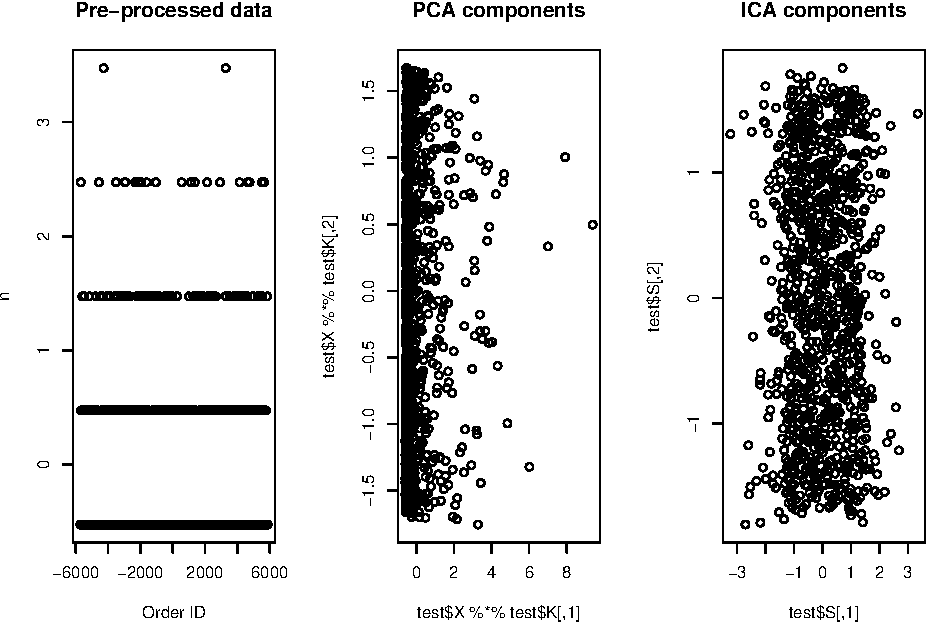
\includegraphics{ICAStatsComps_files/figure-latex/unnamed-chunk-32-1} \end{center}
  
  While the PCA model provides minimal information, the ICA model for the
  superstore data by order ID appears to have separated some particular
  ID's from a massive cluster of orders. These orders could be the most
  atypical in terms of quantity or price, but this separation indicates
  the effectiveness of the ICA model on the data in general.
  
  \subsection{Run 1000 fastICA
  Iterations}\label{run-1000-fastica-iterations}
  
  \begin{Shaded}
  \begin{Highlighting}[]
  \KeywordTok{set.seed}\NormalTok{(}\DecValTok{10}\NormalTok{)}
  \NormalTok{N <-}\StringTok{ }\DecValTok{1000}
  \NormalTok{itF <-}\StringTok{ }\KeywordTok{rep}\NormalTok{(}\OtherTok{NA}\NormalTok{,}\DecValTok{1}\NormalTok{,N)}
  
  \NormalTok{colMax <-}\StringTok{ }\ControlFlowTok{function}\NormalTok{(data) }\KeywordTok{sapply}\NormalTok{(data, max, }\DataTypeTok{na.rm =} \OtherTok{TRUE}\NormalTok{)[}\DecValTok{1}\NormalTok{] }
  \NormalTok{gen_s <-}\StringTok{ }\ControlFlowTok{function}\NormalTok{(N,S)  \{}
    \ControlFlowTok{for}\NormalTok{ (i }\ControlFlowTok{in} \DecValTok{1}\OperatorTok{:}\NormalTok{N) \{}
  \NormalTok{    test <-}\StringTok{ }\KeywordTok{fastICA}\NormalTok{(z1,}\DecValTok{8}\NormalTok{, }\DataTypeTok{alg.typ=}\StringTok{"parallel"}\NormalTok{,}\DataTypeTok{fun=} \StringTok{"logcosh"}\NormalTok{,}\DataTypeTok{row.norm=}\OtherTok{FALSE}\NormalTok{,}\DataTypeTok{maxit=}\DecValTok{5}\NormalTok{,}\DataTypeTok{tol=} \FloatTok{0.0001}\NormalTok{,}\DataTypeTok{verbose=}\OtherTok{TRUE}\NormalTok{)}
  
  \NormalTok{    itF[i] <-}\StringTok{ }\KeywordTok{colMax}\NormalTok{(}\KeywordTok{abs}\NormalTok{(}\KeywordTok{congru}\NormalTok{(S,test}\OperatorTok{$}\NormalTok{S)))}
  
  
  \NormalTok{  \}}
    \KeywordTok{return}\NormalTok{(itF)}
  \NormalTok{\}}
  \end{Highlighting}
  \end{Shaded}
  
  \subsection{Absolute Maxmimum Congruency
  Coefficient}\label{absolute-maxmimum-congruency-coefficient}
  
  \begin{Shaded}
  \begin{Highlighting}[]
  \KeywordTok{kable}\NormalTok{(}\KeywordTok{favstats}\NormalTok{(reps))}
  \end{Highlighting}
  \end{Shaded}
  
  \begin{longtable}[]{@{}lrrrrrrrrr@{}}
  \toprule
  & min & Q1 & median & Q3 & max & mean & sd & n & missing\tabularnewline
  \midrule
  \endhead
  & 4.17e-05 & 0.0069342 & 0.0172902 & 0.0355768 & 0.5157638 & 0.074891 &
  0.1511403 & 1000 & 0\tabularnewline
  \bottomrule
  \end{longtable}
  
  Like with the CPP simulation, the superstore data had to be compared to
  the observations as opposed to the true S. Unsurprisingly, this produces
  a very low coefficient with high standard deviation so does not seem
  inform the analysis in a particularly useful way.
  
  Largely, these two dataset applications may have not been the most
  compelling examples of the power of ICA due to their limited
  dimensionality and lack of complexity to their data structure as a
  whole.
  
  \chapter*{Conclusion}\label{conclusion}
  \addcontentsline{toc}{chapter}{Conclusion}
  
  \setcounter{chapter}{4} \setcounter{section}{0}
  
  \section{Concluding Thoughts}\label{concluding-thoughts}
  
  While Independent Component Analysis can be highly effective on a wide
  range of datasets, its ambiguities regarding particular results and
  relatively difficulty of interpretation explain the lack of widespread
  usage by the Statistical community at large. Even if the key model
  criteria (independence and non-Gaussianity) are met, choosing the
  correct number of components and making sense of the output requires a
  deep understanding of the data.
  
  However,despite the complexity of its application, ICA has proven to be
  an effective method for improving understanding in several fields of
  study. For example, in their study on parallel time series financial
  data, Kiviluoto and Oja discovered how the method successfully revealed
  underlying factors in the retail chain they analyzed. Their findings
  showed the underlying effect of different mangagement on the
  productivity of a given store. The only downside with this analysis
  being that it also demonstrated how ICA modeling calls for ``inspection
  from a domain expert.'' ({\textbf{???}}) Perhaps the best example of
  this need for experts to analyze results is the work done with the ICA
  model on brain imaging data like EEG and MEG. In many ways, ICA has
  proven to be a valuable tool for neuroscience researchers, but this
  application would not be possible with analysis by statisticians alone.
  Although successful understanding of results in this case may always be
  limited to experts, new ICA algorithms with more explicit outputs could
  potentially be developed to improve breadth of its application.
  
  \appendix
  
  \singlespacing
  
  \chapter{}\label{section}
  
  This first appendix includes all of the R chunks of code that were
  hidden throughout the document (using the \texttt{include\ =\ FALSE}
  chunk tag) to help with readability and/or setup.
  
  \subsubsection{In the main Rmd file:}\label{in-the-main-rmd-file}
  
  \begin{Shaded}
  \begin{Highlighting}[]
  \CommentTok{# This chunk ensures that the acstats package is}
  \CommentTok{# installed and loaded. This acstats package includes}
  \CommentTok{# the template files for the thesis and also two functions}
  \CommentTok{# used for labeling and referencing}
  \ControlFlowTok{if}\NormalTok{(}\OperatorTok{!}\KeywordTok{require}\NormalTok{(devtools))}
    \KeywordTok{install.packages}\NormalTok{(}\StringTok{"devtools"}\NormalTok{, }\DataTypeTok{repos =} \StringTok{"http://cran.rstudio.com"}\NormalTok{)}
  \ControlFlowTok{if}\NormalTok{(}\OperatorTok{!}\KeywordTok{require}\NormalTok{(acstats))\{}
    \KeywordTok{library}\NormalTok{(devtools)}
  \NormalTok{  devtools}\OperatorTok{::}\KeywordTok{install_github}\NormalTok{(}\StringTok{"Amherst-Statistics/acstats"}\NormalTok{)}
  \NormalTok{\}}
  \KeywordTok{library}\NormalTok{(acstats)}
  \KeywordTok{library}\NormalTok{(knitr)}
  \KeywordTok{library}\NormalTok{(readr)}
  \KeywordTok{library}\NormalTok{(fastICA)}
  \KeywordTok{library}\NormalTok{(ica)}
  \KeywordTok{library}\NormalTok{(gridExtra)}
  \end{Highlighting}
  \end{Shaded}
  
  \subsubsection{\texorpdfstring{In
  \protect\hyperlink{ref_labels}{}:}{In :}}\label{in}
  
  \chapter{The Second Appendix, for
  Fun}\label{the-second-appendix-for-fun}
  
  \backmatter
  
  \chapter{References}\label{references}
  
  \noindent
  
  \setlength{\parindent}{-0.20in} \setlength{\leftskip}{0.20in}
  \setlength{\parskip}{8pt}
  
  \hypertarget{refs}{}
  \hypertarget{ref-Oja2001}{}
  Aapo Hyvärinen, Juha Karhunen, \& Oja, E. (2001). \emph{Independent
  component analysis}. New York, New York: A Wiley Interscience
  Publication.
  
  \hypertarget{ref-cardoso93}{}
  Cardoso, J. F., \& Souloumiac, A. (1993). Blind beamforming for
  non-gaussian signals. \emph{IEE Proceedings F - Radar and Signal
  Processing}, \emph{140}(6), 362--370.
  \url{http://doi.org/10.1049/ip-f-2.1993.0054}
  
  \hypertarget{ref-icaR}{}
  Helwig, N. E. (2015, August). Independent component analysis.
  \emph{``Proceedings of'' SIGGRAPH 2000}. Retrieved from
  \url{https://cran.r-project.org/web/packages/ica/ica.pdf}
  
  \hypertarget{ref-Oja2000}{}
  Hyvärinen, A., \& Oja, E. (2000). Independent component analysis:
  Algorithms and applications. \emph{``'Independent Component Analysis:
  Algorithms and Applications' Neural Netw. 200}, 411--30.
  
  \hypertarget{ref-izenman2003}{}
  Izenman, A. J. (2003). What is independent component analysis?
  
  \hypertarget{ref-fastICA}{}
  J L Marchini \textless{}marchini@stats.ox.ac.uk\textgreater{}, C. H.
  \textless{}. r, \& \textless{}ripley@stats.ox.ac.uk\textgreater{}, B. D.
  R. (2017, June). FastICA algorithms to perform ica and projection
  pursuit. Retrieved from
  \url{https://cran.r-project.org/web/packages/fastICA/fastICA.pdf}
  
  \hypertarget{ref-walmartdata}{}
  Kaggle/Walmart. (2017, September). Walmart recruiting - store sales
  forecasting. Retrieved from
  \url{https://www.kaggle.com/c/walmart-recruiting-store-sales-forecasting}
  
  \hypertarget{ref-JADE}{}
  Klaus Nordhausen, J. M., Jean-Francois Cardoso. (2017, January). Blind
  source separation methods based on joint diagonalization and some bss
  performance criteria. \emph{N/A}. Retrieved from
  \url{https://cran.r-project.org/web/packages/JADE/JADE.pdf}
  
  \hypertarget{ref-puigt2011}{}
  Puigt, M. (2011). \emph{A very short introduction to blind source
  separation}. Heraklion, Crete, Greece: Foundation for Research;
  Technology -- Hellas Institute of Computer Science.
  
  \hypertarget{ref-storedata}{}
  Tableau. (2017, September). Sample - superstore sales. Retrieved from
  \url{https://community.tableau.com/docs/DOC-1236}


  % Index?

\end{document}

